In this chapter some concepts related to the intersection of the two areas of this research are presented: the computer science applied to an electrical engineering problem, i.e., the use of formal verification methodology to perform automated verification and optimal sizing of stand-alone solar PV systems.

First, the concept of formal verification is introduced as background to understanding how a methodology that performs (mainly) bug detection can be used to validate a design sizing or to obtain an optimal solution of PV systems.

And secondly, how a solar PV system can be modelled in order to be validated or optimized by the formal verification methodology.

\section{Formal Methods, Formal Design and Formal Verification}

Formal methods are system design techniques that use rigorously specified mathematical models to validate systems, most notably (and known for) software and hardware systems~\cite{Collins98}. In contrast to other design systems, formal methods use mathematical proof as a complement to system testing in order to ensure correct behavior. With increasing scale and complexity, and safety becomes a more important issue, the formal approach to system design offers another level of insurance.

Formal methods differ from other design systems through the use of formal verification schemes, the basic principles of the system must be proven correct before they are accepted~\cite{Bowen93}. Traditional system design has used extensive testing to verify behavior, but testing is capable of only finite conclusions. Dijkstra and others have demonstrated that tests can only show the situations where a system won't fail, but cannot say anything about the behavior of the system outside of the testing scenarios~\cite{Bentley99}. In contrast, once a theorem is proven true it remains true.

Prior the 80's, mainly deductive verification was used as formal method, with the use of axioms and proving rules to demonstrate the correctness of the system. The original focus was to verify critical systems based on the premise that 'if system is important, must spend the enough time to verify it'~\cite{Lowry1998}. Worth to mention that back in time, formal methods were initially performed by hand.

It is very important to note that formal verification does not avoid the need for testing~\cite{Bowen95}. Formal verification cannot fix bad assumptions in the design, but it can help identify errors in reasoning which would otherwise be left unverified. In several cases, engineers have reported finding flaws in systems once they reviewed their designs formally~\cite{Kling95}.

A formal design can be summarized as a three step process, as described below~\cite{Collins98}:

\begin{itemize}
\item Formal Specification: During the formal specification phase, the engineer rigorously defines a system using a modelling language. Modeling languages are fixed grammars which allow users to model complex structures out of predefined types (are rigorously defined). This process of formal specification is similar to the process of converting a word problem into algebraic notation and help engineers to clearly define their problems, goals and solutions. Several engineers who have used formal specifications say that the clarity that this stage produces is a benefit in itself~\cite{Kling95}.
\item Verification: As stated above, formal methods differ from other specification systems by their heavy emphasis on provability and correctness. By building a system using a formal specification, the designer is actually developing a set of theorems about his system. By proving these theorems correct, the formal verification ensures that the modelled system has an intended behavior. Verification is a difficult process, largely because even the simplest system has several dozen theorems, each of which has to be proven. Given the demands of complexity and Moore's law, almost all formal systems use an automated theorem proving tool of some form~\cite{Collins98}. That is the origin of 'automated verification' definition. These tools can prove simple theorems, verify the semantics of theorems, and provide assistance for verifying more complicated proofs and with feedback about the trace of the error (in order to correct the system and the specification of it).
\item Implementation: Once the model has been specified and verified, it is implemented by converting the specification into code.

\end{itemize}




%Formal methods are viewed with a certain degree of suspicion. While formal methods research has been progressing since 1960's, formal methods are only being slowly accepted by engineers. There are several reasons for this, but most of the problems seem to be a result of misapplication. Most formal systems are extremely descriptive and all-encompassing, modeling languages have generally been judged by their capacity to model anything. Unfortunately, these same qualities make formal methods very difficult to use, especially for engineers untrained in the type theory needed for most formal systems.[Bowen93]
%
%Conversely, it is apparent that some form of formal specification is necessary: complex systems require formal models. In addition,the mathematics required for formal methods is becoming a more prominent fixture of engineering curricula, engineering schools in Europe are already requiring courses in VDM, Z and similar formal specifications. Ultimately, formal methods will acquire some form of acceptance, but compromises will be made in both directions: formal methods will become simpler and formal methods training will become more common.
%
%Key Concepts
%Provability And Automated Verification
%Formal methods are distinguished from other specification systems by their emphasis on correctness and proof, which is ultimately another measure of system integrity. Proof is a complement, not a substitute, for testing. Testing is an important part of guaranteeing any system's fitness, but it is finite. Testing cannot demonstrate that a system operates properly; it can only demonstrate that the system works for the tested cases. Because testing cannot demonstrate that the system should work outside the tested cases, formal proof is necessary.
%
%Formally proving computer systems is not a new idea. Knuth and Dijkstra have written extensively on the topic, although their methods of proof are based on the traditional mathematical methods. In pure sciences, proofs are verified through extensive peer review before publication. Such techniques are time-intensive and less than perfect; it isn't unusual for a published proof to contain a flaw. Given the cost and time requirements of systems engineering, traditional proving techniques are not really applicable.
%
%Because of the costs of hand verification, most formal methods use automated theorem proving systems to verify their designs. Automated theorem provers are best described as mathematical CAD tools: they can prove simple propositions and automatically and provide assistance for verifying more complex theorems.
%
%Benefits Of Formal Models
%Formal methods offer additional benefits outside of provability, and these benefits do deserve some mention. However, most of these benefits are available from other systems, and usually without the steep learning curve that formal methods require.
%
%Discipline: By virtue of their rigor, formal systems require an engineer to think out his design in a more thorough fashion. In particular, a formal proof of correctness is going to require a rigorous specification of goals, not just operation. This thorough approach can help identify faulty reasoning far earlier than in traditional design.[Bowen95]
%The discipline involved in formal specification has proved useful even on already existing systems. Engineers using the PVS system, for example, reported identifying several microcode errors in one of their microprocessor designs.[Miller95]
%
%Precision: Traditionally, disciplines have moved into jargons and formal notation as the weaknesses of natural language descriptions become more glaringly obvious. There is no reason that systems engineering should differ, and there are several formal methods which are used almost exclusively for notation.[Bowen93]
%For engineers designing safety-critical systems, the benefits of formal methods lie in their clarity. Unlike many other design approaches, the formal verification requires very clearly defined goals and approaches. In a safety critical system, ambiguity can be extremely dangerous, and one of the primary benefits of the formal approach is the elimination of ambiguity.[Kling94].
%
%Weaknesses Of Formal Methods
%: Bowen points out that formal methods are generally viewed with suspicion by the professional engineering community, and the propensity of tentative case studies and advocacy papers for the formal approach would seem to support his thesis [Bowen93]. There are several reasons why formal methods are not used as much as they might be, most stemming from overreaching on the part of formal methods advocates.
%Expense:Because of the rigor involved, formal methods are always going to be more expensive than traditional approaches to engineering. However, given that software cost estimation is more of an art than a science, it is debatable exactly how much more expensive formal verification is. In general, formal methods involve a large initial cost followed by less consumption as the project progresses; this is a reverse from the normal cost model for software development.[Bowen93]
%
%Limits Of Computational Models:While not a universal problem, most formal methods introduce some form of computational model, usually hamstringing the operations allowed in order to make the notation elegant and the system provable. Unfortunately, these design limitations are usually considered intolerable from a developer's perspective.
%An excellent example comes from SML. Statements of proof in SML depend on a purely functional programming model: all data is passed through the parameter/return mechanism of a function, no side effect alterations, modifications of global variables or the like is allowed [Paulson96]. Handling side effects and other aberrancies are a requirement for any system involving input, network operations or other systems which require interrupts, meaning that SML's model is, to some extent, broken.
%
%Usability:Traditionally, formal methods have been judged on the richness of their descriptive model. That is, 'good' formal methods have described a wide variety of systems, and 'bad' formal methods have been limited in their descriptive capacities. While an all-encompassing formal description is attractive from a theoretical perspective, it invariably involved developing an incredibly complex and nuanced description language, which returns to the difficulties of natural language. Case studies of full formal methods often acknowledge the need for a less all-encompassing approach.[Miller95]
%Arguably, many of these failures can be attributed to overreaching on the part of formal methods advocates. This reasoning has led to the lightweight approach to formal specification.
%
%The Lightweight Approach
%The flaws in formal specifications have been heavily focused on in the past few years, leading to several alternate approaches. The traditional view of formal methods as all-encompassing highly abstracted schemes has led to formal methods being all-encompassing, extremely rigorous, and very expensive. While theoretically appealing, formal methods have generally been ignored by engineers in the field.
%The lightweight approach to formal design recognizes that formal methods are not a panacea: there are areas where formal methods are useful, and areas where a formal specification will accomplish nothing. In a lightweight design, formal methods are used in specific locations, and different formal methods may be used in different subsystems, ideally playing to the strengths of each method [Easterbrook 98]. In such a system, Petri Nets might be used to describe the communications protocol, and a LARCH system might be used to model the data storage. For other parts of the system, formal specifications might be avoided entirely: for example, the user interface may be refined using a rapid prototyping system and client interviews.
%
%The lightweight approach is a traditional engineering compromise, and there is a tradeoff. As formal methods become more common, engineers will have to learn type theory, modern algebra and proof techniques. Ultimately, engineers will have to think more like mathematicians.

\section{Project Validation, Automated Verification and Synthesis Using Model Checking}
\label{sec:AutomatedVerification}
%%%%%%%%%%%%%%%%%%%%%%%%%%%%%%%%%%%%%%%%%%%%%%%%%%%%%%%%

%\section{Automated Verification }
It is necessary to keep in mind that validation is the process of determining whether a design meets the needs of the user, whereas verification is the process of determining whether a design meets a set of requirements, specifications, and regulations.  

If the requirements, specifications, and regulations are given in a formal language, then it may be possible to automate verification, resulting in a process known as formal verification. Verification may form part of a validation process, but in general, validation cannot be formalized because it relates a system design to intent.  

Simulation may also be used for validation, but it is more problematic for verification. In order to use simulation for verification, it is necessary to ensure adequate coverage of operating conditions, scenarios, and system inputs. 

Testing can also be used for validation, but for the same reasons, it too is problematic for verification.
 
According \cite{Clarke2008}, verification procedure is an intelligent exhaustive search of the state space of the design. In addition, according to \cite{Forejt2011}, formal verification is a systematic approach that applies mathematical reasoning to obtain guarantees about the correctness of a system. One successful method in this domain is model checking.

\subsection{Model Checking}
  
Model checking is an automatic verification technique, as defined by \cite{Clarke2008}. Model checking was originally developed reasoned about finite state of concurrent systems, nowadays is mainly used to hardware and software verification, but can be applied to any kind of system. 

The process of model checking can be divided in three components: modeling, specification, and verification method. 

\begin{itemize}
\item In modeling, a model (normally mathematical) of the system is created; 
\item In specification, normally a list of properties to be satisfied by the system is stablished, i.e., the requirements, as reliability to performance for example. \item Normally is expressed in temporal logic form ($CTL$); 
\item The model checking is the verification method itself. 
\end{itemize}

The model checking algorithm can be described as:  

\begin{itemize}
\item Given the model $ 'M' $ and a $CTL$ formula $ \phi $ as input;  
\item Model checking algorithm provides all the states of model $ M $ which satisfies $ \phi $;  
\item It returns $YES$ if $ \phi $ is $TRUE$, or returns $NO$ if $ \phi $ is $FALSE$.  

\end{itemize}
Specifically at the $FALSE$ situation, the algorithm returns a counterexample that is useful as diagnostic of the system, in order to discover in which situation the model is violated. \cite{Clarke2008} consider that the most important advantage of the use of model checking.  
 
Among the other advantages can be listed: there is no need of proofs (the algorithm is not a deductive procedure), there is no problem with partial specifications of the system, logics can easily express many concurrency properties, is fast (compared to other rigorous methods such as interactive theorem proving). However, there is a main disadvantage of model checking: the state explosion problem. 

The model checking problem can be defined as shown in \cite{Clarke2008}: 

\begin{itemize}
\item Let $M$ be a Kripke structure (i.e., state transition graph);
\item $f$ be the specification in temporal logic (a formula);
\item Find all states $s$ of $M$ such that $M , s \models f$
\end{itemize}

Fig. \ref{fig:modelcheckstruc} shows the structure of a typical model checking system. A preprocessor extracts a state transition graph from a system (program or circuit).

\begin{figure}[h]
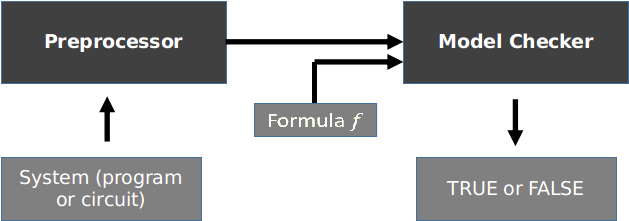
\includegraphics[width=0.8\textwidth]{modelcheckstruc}
\centering
\caption{Model Checker structure. Source: \cite{Clarke2008}.}
\label{fig:modelcheckstruc}
\end{figure}

Here it is worth to mention that the term "model" is not the meaning taken from the dictionary. The problem is not dealing with an abstraction of the actual system under study. 

The Fig. \ref{fig:systemverif} shows the process to convert a real system to a model in order to be verified by a model checking. 

\begin{figure}[h]
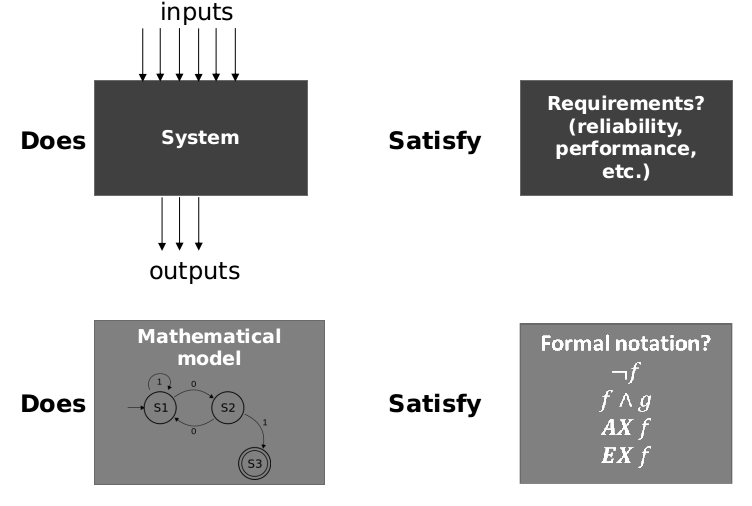
\includegraphics[width=0.8\textwidth]{systemverif}
\centering
\caption{From real system verification to model checking. Source: adapted from \cite{Clarke2008}.}
\label{fig:systemverif}
\end{figure}

In order to solve the problem of state explosion, many different techniques were developed at the last decades. One of the promising is the Bounded Model Checking (BMC). 

BMC is a method that checks the model up to a given path in the path length. BMC algorithms traverses a finite state machine for a fixed number of steps, , and checks whether violation occurs with this bound. It uses fast SAT solvers, where SAT means satisfiability. 

SAT problem, as defined by \cite{Clarke2008}, is a problem of determining if there are certain conditions or interpretation that satisfy a given Boolean expression. SAT solvers are used in BMC, such that if there are some Boolean function, the solver would search the model for conditions (value of variables) that would make the formula $TRUE$. If SAT Solver find a substitution for the formula/function then the substitute induces a counterexample.  

%%CBMC is considering the best-known model verification tool to validate code in ANSI-C and C++, as can be seen in \cite{Kroening}. 
%
%ESBMC is a context-bounded model checker for embedded C/C++ software based on Satisfiability Modulo Theories (SMT) solver, which can use CBMC as front-end.  
The use of SMT, instead of Boolean Satisfiability SAT from the original BMC, comes as an alternative to overcome limitations of the systems modeling, especially considering that the complexity of these is increasing and the SMT method has high level and richer theories than the SAT to represent the models. 

%Although simulation and testing explore possible behaviors and scenarios of a given system, they leave open the question of whether unexplored trajectories may contain a flaw~\cite{ClarkeHV18}. Formal verification conducts an exhaustive exploration of all possible behaviors; when a design is said to be ``correct'' by a formal verification method, it implies that all behaviors have been explored; questions regarding adequate coverage or missed behavior becomes irrelevant~\cite{Clarke2012}. Formal verification is a systematic approach that applies mathematical reasoning to obtain guarantees about the correctness of a system; one successful method in this domain is model checking~\cite{Clarke2012}. 

At this work will be evaluated three state-of-the-art model checkers to formally verifying and synthesize PV designs w.r.t. user requirements.

%%%%%%%%%%%%%%%%%%%%%%%%%%%%%%%%%%%%%%%%%%%%%%%%%%%%%%%%
\subsection{CBMC}
%%%%%%%%%%%%%%%%%%%%%%%%%%%%%%%%%%%%%%%%%%%%%%%%%%%%%%%%

The C Bounded Model Checker (CBMC) falsifies assertions in C programs or proves that they are safe if a completeness threshold is given~\cite{Kroening}. CBMC implements a bit-precise translation of a C program, annotated with assertions and with loops unrolled up to a given depth, into a logical formula. If the formula is satisfiable, then a failing execution that leads to a violated assertion exists~\cite{Kroening}. 

CBMC's verification flow can be summarized in three stages: 

\begin{itemize}
\item Front-end: scans, parses and type-checks C code; it converts control flow elements, such as \textit{if} or \textit{switch} statements, loops and jumps, into equivalent guarded \textit{goto} statements, thus aiming to reduce verification effort; 
\item Middle-end: performs symbolic execution by eagerly unwinding loops up to a fixed bound, which can be specified by the user on a per-loop basis or globally, for all loops and finally; 
\item Back-end: supports SAT and SMT solvers to discharge verification conditions.
\end{itemize}


%%%%%%%%%%%%%%%%%%%%%%%%%%%%%%%%%%%%%%%%%%%%%%%%%%%%%%%%
\subsection{ESBMC}
%%%%%%%%%%%%%%%%%%%%%%%%%%%%%%%%%%%%%%%%%%%%%%%%%%%%%%%%

The Efficient SMT-based Bounded Model Checker (ESBMC) is a bounded and unbounded model checker for C programs~\cite{esbmc2018}, which supports the verification of LTL properties with bounded traces~\cite{DBLP:journals/sosym/MorseCN015}. 

ESBMC's verification flow can be summarized in three stages: 

\begin{itemize}
\item A front-end that can read and compile C code, where the system formal specification is first handled; 
\item Preprocessing steps to deal with code representation, control flow and unwinding of loops, and model simplification, thereby aiming to reduce verification effort; and finally 
\item The SMT solving stage, where all constraints and properties of the system are encoded into SMT and checked for satisfiability.
\end{itemize}
 
ESBMC exploits the standardized input language of SMT solvers (SMT-LIB\footnote{http://smtlib.cs.uiowa.edu/} logic format) to make use of a resource called \textit{assertion stack}~\cite{Morse2015}. This enables ESBMC, and the respective solver, to learn from previous checks, thus optimizing the search procedure and potentially eliminating a large amount of formula state space to be searched, because it solves and disregards data during the process, incrementally. This technique is called ``incremental SMT''~\cite{DBLP:journals/fac/SchrammelKBMTB17} and allows ESBMC to reduce the memory overhead, mainly when the verified system is complex and the computing platform does not have large amount of memory to deal with the entire design space state.

%%%%%%%%%%%%%%%%%%%%%%%%%%%%%%%%%%%%%%%%%%%%%%%%%%%%%%%%
\subsection{CPAchecker}
%%%%%%%%%%%%%%%%%%%%%%%%%%%%%%%%%%%%%%%%%%%%%%%%%%%%%%%%

Automatic program verification requires a choice between precision and efficiency. The more precise a method, the fewer false positives it will produce, but also the more expensive it is, and thus applicable to fewer programs. 

Historically, this trade-off was reflected in two major approaches to static verification: program analysis and model checking. In order to experiment with the trade-off, and in order to be able to set the dial between the two extreme points, Configurable Program Analysis (CPA) provides a conceptual basis for expressing different verification approaches in the same formal setting. 

The CPA formalism provides an interface for the definition of program analyses. Consequently, CPAchecker provides an implementation framework that allows the seamless integration of program analyses that are expressed in the CPA framework. The comparison among different approaches in the same experimental setting is intended to be easy and the experimental results are expected to be more meaningful~\cite{Beyer2011}. Related to the architecture, the central data structure is a set of control-flow automata (CFA), which consists of control-flow locations and control-flow edges. 

The CPA framework provides interfaces to SMT solvers and interpolation procedures~\cite{Beyer2011}. Currently, CPAchecker uses MathSAT as SMT solver; and CSIsat and MathSAT as interpolation procedures~\cite{Beyer2011}. %CPAchecker performs reachability analysis and operates on an object of the abstract data type CPA, i.e., the underlying verification algorithm applies operations from the CPA interface without knowing which concrete CPA it is analyzing. For most configurations, the concrete CPA will be a composite CPA, which implements the combination of different CPAs. \textcolor{red}{It is unclear what a CPA is.}
%In software verification, it is usual to take a considerable amount of effort to convert a verification idea into actual experimental results and CPAchecker aims to accelerate this process~\cite{Beyer2011}.

//////Begin optimization
%-----------------------------------------------------------
\subsection{CEGIS and Program Synthesis}
\label{sec:ProgramSynthesis}
%-----------------------------------------------------------

The basic idea of program synthesis is to automatically construct a program $P$ that satisfies a correctness specification $\sigma$. In particular, program synthesis is automatically performed by engines that use a correctness specification $\sigma$, as starting point, and then incrementally produce a sequence of candidate solutions that partially satisfy $\sigma$~\cite{Abateetal2017}. As a result, a given candidate program $p$ is iteratively refined, in order to match $\sigma$ more closely. CEGIS represents one of the most popular approaches to program synthesis that are currently used in practice for CPS~\cite{Abateetal2017}, whose basic architecture is illustrated in Figure~\ref{Counter-Example-Guided-Inductive-Synthesis} and has close connections to algorithmic debugging using counterexamples and abstraction refinement~\cite{Alur}. 

\begin{figure}[h]
	\centering
	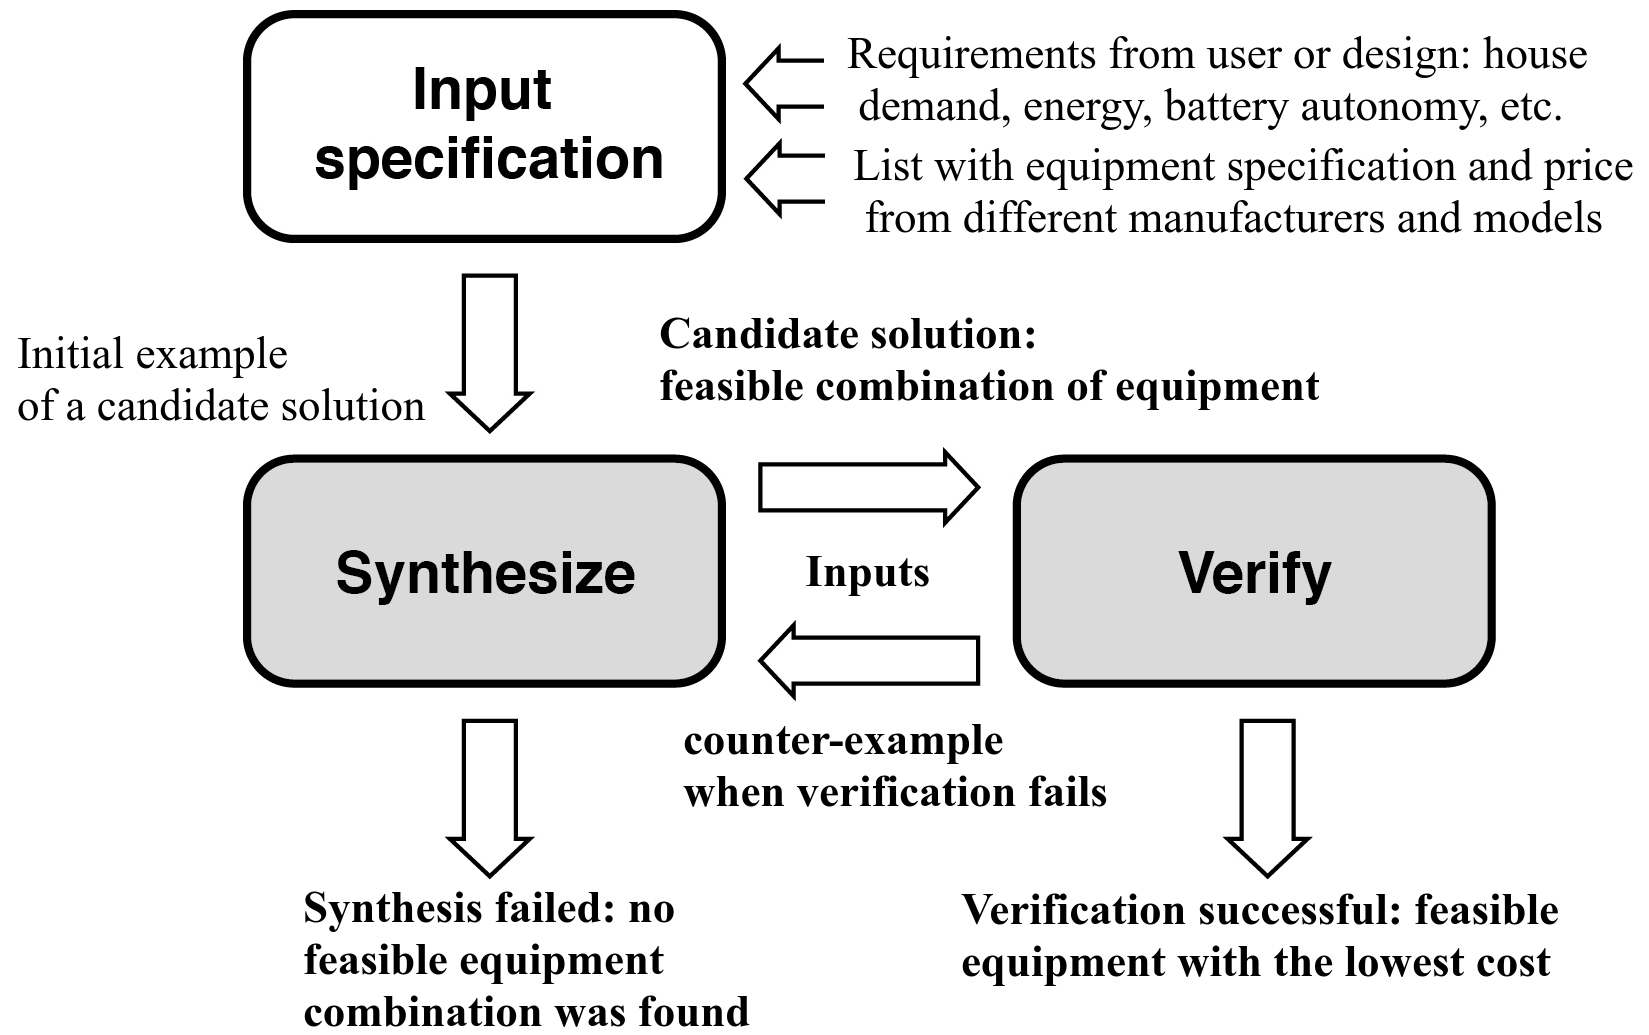
\includegraphics[width=0.75\columnwidth]{fig2_rev.jpg}
	\caption{CEGIS applied to PV system sizing.}
	\label{Counter-Example-Guided-Inductive-Synthesis}
\end{figure}

The correctness specification $\sigma$ provided to our program synthesizer is of the form $\exists \vec{F} .  \forall \vec{x}.  \sigma(\vec{x}, \vec{F})$, where $\vec{F}$ ranges over functions, $\vec{x}$ ranges over ground terms, and $\sigma$ is a quantifier-free (QF) formula typically supported by SMT solvers. The ground terms are interpreted over some finite domain $\mathcal{D}$, where $\mathcal{D}$ can be encoded using the SMT's bit-vectors part. Examples of specification used by our method include house demand, energy, and battery autonomy; we also provide a list of equipment specification and price from different manufacturers and models.

In Figure~\ref{Counter-Example-Guided-Inductive-Synthesis}, regarding traditional CEGIS method, the phases {\sc Synthesize} and {\sc Verify} interact via a finite set of test vectors {\sc inputs}, which is incrementally updated. Given the correctness specification $\sigma$, the {\sc Synthesize} procedure tries to find an existential witness $\vec{F}$ satisfying the specification $\sigma(\vec{x}, \vec{F})$, for all $\vec{x}$ in {\sc inputs} (as opposed to all $\vec{x} \in \mathcal{D}$). If {\sc Synthesize} succeeds in finding a witness~$\vec{F}$, the latter is a candidate solution (i.e., feasible combination of equipment) to the full synthesis formula, which is passed to {\sc Verify} in order to check whether it is a proper solution ({\it i.e.}, $\vec{F}$ satisfies the specification $\sigma(\vec{x}, \vec{F})$ for all $\vec{x}\in\mathcal{D}$). If this is the case, then the algorithm terminates, i.e., we have found a feasible equipment with the lowest cost; otherwise, in the CEGIS traditional method, additional information is provided to the phase {\sc Synthesize}, in the form of a new counterexample that is added to the {\sc inputs} set and the loop iterates again.

One may notice that each iteration of the traditional CEGIS loop adds a new input to the finite set $\text{\sc inputs}$, which is then used for synthesis.  Given that the full set of inputs $\mathcal{D}$ is finite because we use bit-vector expressions, this means that the refinement loop can only iterate over a finite number of times; however, {\sc Synthesize} may conclude that no candidate solution obeying $\sigma$ for the finite set $\text{\sc inputs}$ exists and our synthesis engine can then conclude that no feasible equipment combination was found.

\section{Solar Photovoltaic System }
According to \cite{Roy}, a PV system is designed to give the electric supply to a load. This load can be either Alternate Current (AC) type or Direct Current (DC) type. Electric supply can be needed either in daytime or evening time (in particular cases, in both times). The most basic PV system can give supply only in daytime.  For night hours or rainy days, one needed to have batteries, where power can be stored and used \cite{Gules}. 

PV systems are broadly classified into three distinct types, as described by \cite{Mohanty}: 

\begin{itemize}
\item Standalone systems, where the energy is generated and consumed in the same place and which does not interact with the main grid. Normally, the electricity consuming/utilizing device is part of the system, i.e., solar home systems, solar street lighting system, solar lanterns, and solar power plants; 
\item Grid-connected systems, where the solar PV system is connected to the grid. The grid-connected system can be either a grid-tied system, which can only feed power into the grid and such system cannot deliver power locally during blackouts and emergencies since these systems have to be completely disconnected from the grid and have to be shut down as per national and international electrical safety standards. Some grid-connected PV systems, with energy storage, can also provide power locally in an islanding mode; 
\item Solar PV hybrid system: In a hybrid system, another source(s) of energy, such as wind, biomass or diesel, can work together with the solar PV system to provide the required demand. In such type of system, main objective is to bring more reliability into the overall system at an affordable way by adding one or more energy sources.
\end{itemize}
 
Specifically concerning isolated communities, depending on the type of load, cost, resources availability, and requirements of the load, standalone systems can be split into several categories, which are described in this section. As the goal of this Thesis is just the solutions aimed to isolated/ off-grid application, therefore it is not considered the on-grid or hybrid configurations.
 
There is a resource, called maximum power point tracking (MPPT), which is an electronic control mechanism that maintains the PV operating in a voltage that correspond to the voltage of maximum power, which maximizes the transfer of power and avoiding lost at the PV cells \cite{Pinho}. That resource is found at modern PV systems and is strongly indicated due to its advantages.

\subsection{Unregulated standalone PV system with DC load }
Usually this type of system is for low power applications, as defined by \cite{Roy}. The PV system is directly connected to the load without any MPPT controller, as shown at Fig.\ref{fig:unregSPV}. At night hours, the system will not provide any supply because of the absence of the battery. 
 
\begin{figure}[h]
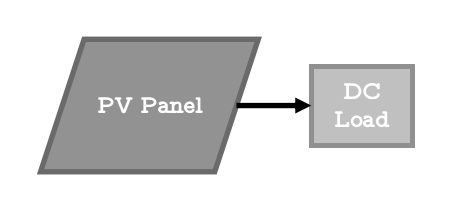
\includegraphics[width=0.6\textwidth]{unregulatedSPV.png}
\centering
\caption{Unregulated standalone SPV system with DC load. Source: \cite{Roy}.}
\label{fig:unregSPV}
\end{figure}

\subsection{Regulated standalone PV system with DC load}
It is similar to unregulated standalone system with DC load, but the main difference between this and the previous one is that this system requires a MPPT technique, as illustrated by Fig.\ref{fig:regSPV1}. Usually system with MPPT should have battery; otherwise, extra power will be waste.

\begin{figure}[h]
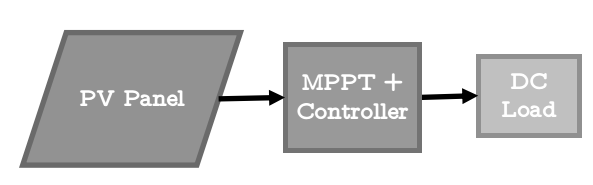
\includegraphics[width=0.8\textwidth]{regulatedSPV1.png}
\centering
\caption{Regulated standalone SPV system with DC load. Source: \cite{Roy}.}
\label{fig:regSPV1}
\end{figure}

\subsection{Regulated standalone system with battery and DC load}
Configuration with PV array, battery, MPPT and DC load, as shown in Fig.\ref{fig:regSPV2}. Battery is used to store the extra power of PV system. A charge controller is necessary for this type of system because the useful life of the battery is less than that of the PV module. Extra charging and deep discharging can reduce the battery life \cite{Kim}. 

\begin{figure}[h]
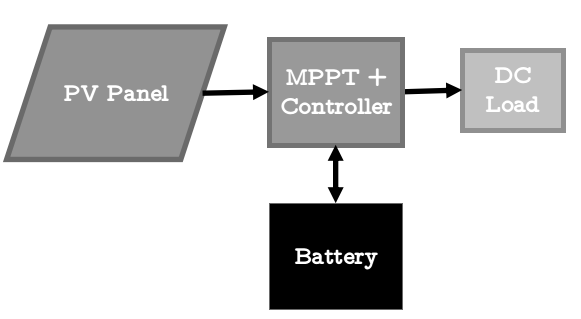
\includegraphics[width=0.8\textwidth]{regulatedSPV2.png}
\centering
\caption{Regulated standalone SPV system with battery DC load. Source: \cite{Roy}.}
\label{fig:regSPV2}
\end{figure}

According to \cite{Pinho}, PV systems that are used to feed loads with low variation on the consumption can be sized to operate without the controller. That is called of self-regulated standalone PV system with battery. However, the voltage from the PV panel must be compatible with the batteries voltage. Normally, the bank of batteries are oversized related to the PV panel and to the load. The drawback is the operation of the batteries, normally overloaded or with excessive discharges (that can damage the batteries).

\subsection{Regulated standalone system with battery, AC load}
This system is similar to the previous one, but here AC load draws the power from PV system and, because of the AC load, an inverter (DC to AC converter) is required, as seen in Fig.\ref{fig:regSPV3}. This solution has an increase of cost because has more equipments. However, the AC availability brings the advantage of a higher number of AC appliances to use at the houses or consumer units. That configuration is the focus of the present thesis since it is the most common nowadays all over the world, when off-grid or isolated regions is the target. \textcolor{red} { Alternative??? Specifically for remote rural areas of developing countries or places where the grid extension is not feasible,}
%stand-alone systems are one the most used solutions, and 
% depending on the type of load, cost, resources availability, and requirements of the load, 
%stand-alone systems 
%can be split into several categories. However, 
the most suitable configuration is the regulated stand-alone system with battery and AC load.

\begin{figure}[h]
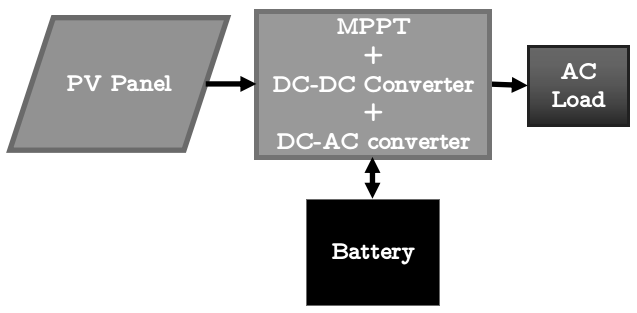
\includegraphics[width=0.8\textwidth]{regulatedSPV3.png}
\centering
\caption{Regulated standalone system with battery, AC load. Source: \cite{Roy}.}
\label{fig:regSPV3}
\end{figure}

\subsection{Design and Validation of a Solar photovoltaic system}
The design and validation of a SPV system can be done by hand or with the aid of a software tool. 

In order to address different aspects of project system and systems design, there is a myriad of public domain and commercial software available for the SPV market. According to \cite{Brooks}, the capabilities of these tools range from simple solar resource and energy production estimative, to site survey and system design tools, to complex financial analysis software (with optimization). Some tools also provide support to rebate programs applications and tax incentives (specific to each country or region), while other programs and worksheets focus on the technical aspects of system sizing and design.
 
Manufacturers and integrators have yet their proprietary software to perform inverter string sizing and various system sizing and design tools, with the drawback to just include their own products among the possibilities of choice. 
In this study, the most popular tools are presented: 

\begin{itemize}
\item PVWatts 
\item SAM
\item Homer
\item RETScreen
\item Hybrid2
\end{itemize}

\subsubsection{PVWatts Calculator}
According to \cite{Freeman} and \cite{NRELDobos}, it is a web application developed by the National Renewable Energy Laboratory (NREL), which estimates the electricity production of a grid-connected roof- or ground-mounted photovoltaic system based on a few inputs. According to \cite{NRELDobos}, to use the calculator, it is necessary to provide information about the system's location, basic design parameters, and system economics. PVWatts calculates estimated values for the system's annual and monthly electricity production, and for the electricity monetary value. This tool is suitable for very preliminary studies of a potential location for a photovoltaic system that uses crystalline silicon or thin film photovoltaic modules. The production estimates that PVWatts computation do not account for many factors that are important in the design of a photovoltaic system, therefore it is necessary support of an energy expert. The calculator estimates the monthly and annual electricity production of a photovoltaic system using an hour-by-hour simulation over a period of one year. To represent the system's physical characteristics, PVWatts requires values for six inputs: System DC size; Module type; Array type; System losses; Array tilt angle; Array azimuth angle.

\subsubsection{SAM}
SAM or System Advisor Model is a software from the U.S. Department of Energy and National Renewable Energy Laboratory. According to \cite{NRELBlair} and \cite{Cameron2008}, SAM is intended to help users to determine whether the model meets their project constraints/specifications, and (also) to provide information for readers who do not plan to use the model, but want to learn about its capabilities. SAM is a performance and financial model designed to facilitate decision making for people involved in the renewable energy industry: Project managers and engineers; Financial and policy analysts; Technology developers; and Researchers. SAM makes performance predictions and cost of energy estimates for grid-connected power projects based on installation and operating costs and system design parameters that you specify as inputs to the model. Projects can be either on the customer side of the utility meter, where they buy and sell electricity at retail rates, or on the utility side of the meter, where they sell electricity at a price negotiated through a power purchase agreement. SAM is an electric power generation model and assumes that the renewable energy system delivers power either to an electric grid, or to a grid-connected building or facility to meet electric load. It does not model thermal energy systems that meet a thermal process load. As mentioned in \cite{NRELBlair}, SAM does not model isolated or off-grid power systems, and does not model systems with electricity storage batteries.

\subsubsection{HOMER}
As defined in \cite{HOMER}, actually is a set of two tools: HOMER Legacy and HOMER Pro. HOMER is an acronym for Hybrid Optimization Model for Multiple Energy Resources. HOMER Legacy is the original HOMER software version created at the National Renewable Energy Laboratory (NREL). HOMER Legacy is a free computer model that simplifies the task of evaluating design options for both off-grid and grid-connected power systems for remote, stand-alone, and distributed generation applications. HOMER's optimization and sensitivity analysis algorithms allow the user to evaluate the economic and technical feasibility of a large number of technology options. Since 2016 Homer Legacy can be found at HOMER web site, but only available for students and nonprofit organizations, as defined in \cite{HOMER}, and has not support available. At the short-time only the commercial version will remain.
 
The commercial version (paid), called HOMER Pro, as defined in \cite{Swarnkar}, is a tool for optimizing micro-grid design in all sectors, from village power and island utilities to grid-connected campuses and military bases. HOMER Pro put together three tools in one product: optimization, simulation, and sensitivity analysis. HOMER Pro provides the detailed rigor of chronological simulation and optimization in a model that is intended to be easy to use. It is adaptable to a wide variety of projects. For a village or community-scale power system, HOMER can model both the technical and economic factors involved in the project. For larger systems, HOMER can provide an overview that compares the cost and feasibility of different configurations. Chronological simulation is essential for modeling variable resources, such as solar and wind power and for combined heat and power applications, where the thermal load is variable. HOMER's sensitivity analysis helps determine the potential impact of uncertain factors such as fuel prices or wind speed on a given system. 

\subsubsection{RETScreen}
As mentioned in \cite{Pradhan}, RETScreen is a decision-support tool designed to help decision makers and energy professionals to evaluate the financial viability of renewable energy, energy efficiency, and/or co-generation projects.

RETScreen models various types of renewable energy technologies (RETs), allowing for comparisons between technology options. The software can be used to evaluate benefits from both clean energy production from power generation projects and savings through energy efficiency projects, accounting for project costs, greenhouse gas emission reductions, and financial risk. The software is freely distributed (but with restrictions to save work or print), and had three different versions:

\begin{itemize}
\item RETScreen 4 (discontinued, requires Microsoft Excel to run); 
\item RETScreen Software Suit, which includes the RETScreen 4 and a Windows-based graphical software that allows project owners to verify the ongoing energy performance of their facilities (discontinued in 2013);
\item And the actual (2016) RETScreen Expert, which allows users to evaluate energy investments over an entire project life-cycle (including benchmarking, feasibility, and performance analysis) in a fully integrated way, and within one software platform. However, this version works is only Windows-based. This version has a complete paid version, in an annual subscription way.
\end{itemize}

As described by \cite{Pradhan}, RETScreen performs a five-step standard analysis: setting and site conditions; energy model; cost analysis; emission analysis, financial analysis, sensitivity, and risk analysis. It is developed and maintained by the Government of Canada, through the CanmetENERGY Varennes Research Centre of Natural Resources; in collaboration with: NASA; Renewable Energy and Energy Efficiency Partnership (REEEP); United Nations Environment Programme (UNEP), and the Global Environment Facility (GEF). RETScreen is available in 36 languages; it is a multi-awarded tool, and includes equipment databases for components manufactured and available worldwide.

\subsubsection{Hybrid2}
The Hybrid2 software package, as described in \cite{Mills}, is a user-friendly tool to perform detailed long-term performance and economic analysis on a wide variety of hybrid power systems. Hybrid2 is a probabilistic/time series computer model, using time series data for loads, wind speed, solar insolation, and temperature; and the power system is designed or selected by the user, in order to predict the performance of the hybrid power system. Variations in wind speed and in load within each time step are factored into the performance predictions. The code does not consider short-term system fluctuations caused by system dynamics or component transients. This program is not supported anymore and according to \cite{UMASS}, probably after the user performs the free download of the tool, it will not work on Windows platforms later than Windows XP, what is a limitation.

Table \ref{table:softwares} summarizes the tools described in this paper.  Where just Hybrid2 do not have technical support; only HOMER, RETScreen and Hybrid2 perform off-grid system or battery backup analysis; all the tools perform solar photovoltaic analysis; and that only HOMER and RETScreen are complete, including economical analysis or even optimization-sensitive analysis. However, only paid version of those softwares have all the features, and they run only at Windows-based operational systems.

\begin{table}[!t]
%% increase table row spacing, adjust to taste
\renewcommand{\arraystretch}{1.3}
% if using array.sty, it might be a good idea to tweak the value of
% \extrarowheight as needed to properly center the text within the cells
\caption{Comparative coverage of reference softwares}
\label{table:softwares}
\centering
%% Some packages, such as MDW tools, offer better commands for making tables
%% than the plain LaTeX2e tabular which is used here.
\begin{tabular}{c | c | c | c | c | c}
\hline
\hline
Characteristic  & \rotatebox{90}{PVWatts} & \rotatebox{90}{SAM} & \rotatebox{90}{HOMER} & \rotatebox{90}{RETScreen } & \rotatebox{90}{Hybrid2}\\
\hline
Support & X & X & X & X &  \\
Off-grid systems &   &   & X & X & X\\
Hybrid systems &  &  & X & X & X\\
Photovoltaics & X & X & X & X & X\\
Batteries &  &  & X & X & X\\
Main technical (T) or economical (E) & T & T & E & E & T \\
Optimization &  &  & X & X &  \\
Sensitive analysis &  &  & X & X & \\
\hline
\hline
\end{tabular}
\end{table}

\subsubsection{Paper Proposal x Reference Tools}
Considering that the focus of this research is on off-grid solutions and supported tools, only HOMER and RETScreen remain for comparative. All tools need some parameters inherently from manufacturer's catalog, so the project starts with manufacturers and integrators tool to define the basic items of the project: panels, inverters, controllers, and batteries. After that, the potential solution is analyzed in another tool to validate or even optimize the solution. Therefore, that is the challenge of this work, i.e., to prove that is possible to use automated verification to validate an off-grid PV solution.

\subsection{Component models for stand-alone PV system }
The main purpose of this section is to describe the models for the elements of a standalone PV system: PV generator, battery, controller, inverter, and load. The modeling of the PV system is based on modular blocks, as illustrated in Fig.\ref{fig:blockdiagram}, from \cite{Hansen}. The modular structure facilitates the modeling of the other system structures and replacing of elements as, for instance, a DC load instead of an AC load. 

\begin{figure}[h]
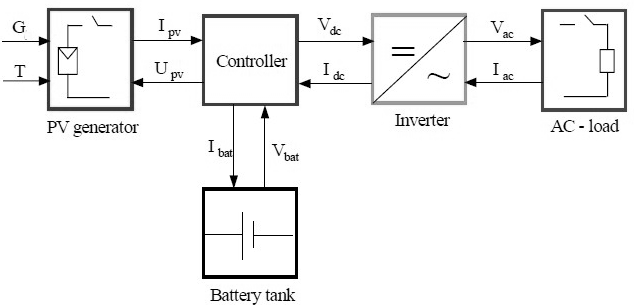
\includegraphics[width=0.95\textwidth]{blockdiagramPVS}
\centering
\caption{Block diagram for the stand-alone PV system. Source: \cite{Hansen}.}
\label{fig:blockdiagram}
\end{figure}

In the literature, there are several mathematical models available for each component of stand-alone PV systems. In this section, the mathematical model for each component of PV system is presented. 

\subsubsection{PV generator (cell, module, array) }
A photovoltaic PV generator is the whole assembly of solar cells, connections, protective parts, and supports. In the present modeling, the focus is only on cell/module/array.
 
The basic element of a PV System is the PV cell, also called a Solar Cell. A PV / Solar Cell is a semiconductor device that can convert solar energy into DC electricity. The semiconductor materials (usually silicon), which are specially treated to form an electric field, positive on one side (backside) and negative on the other (towards the sun). When solar energy (photons) hits the solar cell, electrons are knocked loose from the atoms in the semiconductor material, creating electron-hole pairs \cite{Lorenzo}. If electrical conductors are attached to the positive and negative sides, forming an electrical circuit, the electrons are captured in the form of electric current $ I_{ph} $ (photocurrent).
 
To increase their utility, a number of individual PV cells are interconnected together in a sealed, weatherproof package called Panel (or Module). For instance, a 12 V Panel will have 36 cells connected in series and a 24 V Panel will have 72 PV cells connected in series. In addition, to achieve the desired voltage and current, modules are wired in series and parallel into what is called a PV Array, as shown in Fig.\ref{fig:celmodarray}. The flexibility of the modular PV system allows designers to create PV systems that can meet a wide variety of electrical demands. 

\begin{figure}[h]
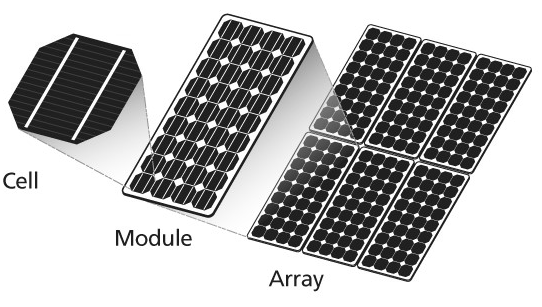
\includegraphics[width=0.95\textwidth]{celmodarray}
\centering
\caption{PV cell, module and array. Source: \cite{SamlexSolar}.}
\label{fig:celmodarray}
\end{figure}

The PV modules are generally rated under standard test conditions (STC), which leads to the following specification by the manufacturers:  solar radiation of 1000 W/m$^{2}$, cell temperature of 25$^{o}$C, and solar spectrum of 1.5. The parameters required for the input of the PV modules are relying on the meteorological conditions of the area to be serviced by photovoltaic solution. However, the climatic conditions are unpredictable due to the random nature of their occurrence \cite{Jakhrani}.
 
These uncertainties lead to either over- or underestimation of energy yield from PV modules. An overestimation up to 40\% was reported as compared to the rated power output of PV modules \cite{Durisch}. The growing demand of photovoltaics technologies led to research in the various aspects of its components from cell technology to the modeling, size optimization, and system performance \cite{Rajanna}, \cite{Badejani}; \cite{Yatimi}, \cite{Ferrari}, \cite{Saloux}, \cite{Hasan}, \cite{King}, \cite{Mellit}. Modeling PV modules is one of the major components responsible for proper functioning of PV systems. However, the estimation of models is affected by various intrinsic and extrinsic factors, which ultimately influence the behavior of current and voltage. Therefore, perfect modeling is essential to estimate the performance of PV modules in different environmental conditions \cite{Jakhrani}.
 
Modeling provides the ways to understand the current, voltage, and power relationships of PV systems.
  
The performance of photovoltaic systems (solar cell/panels), that is, the output current/voltage curve ($I-V$ curve), is usually studied using an equivalent circuit model. This equivalent circuit consists of a current source with one or two diodes connected in parallel, and up to two resistors, one connected in parallel and the other one in series, to take into account energy losses in this model \cite{Cubas}. Based on these electronic components, four basic configurations are normally used when studying photovoltaic systems, as shown by Fig. \ref{fig:equivckt}. 

\begin{figure}[h]
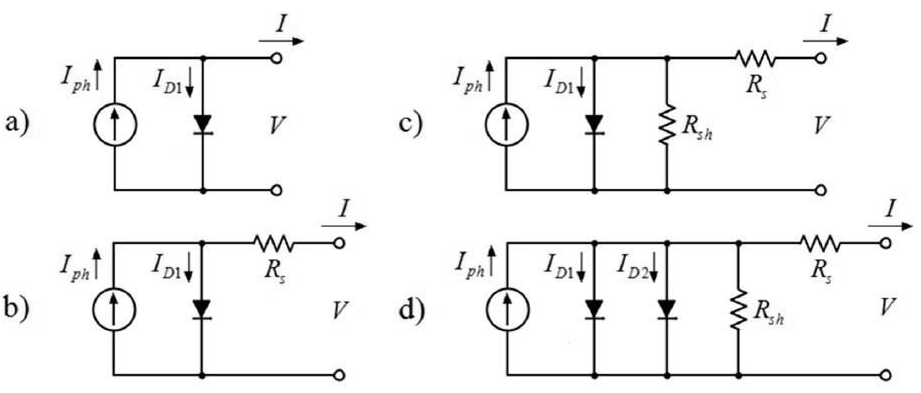
\includegraphics[width=0.95\textwidth]{equivckt}
\centering
\caption{Four different equivalent circuit models: (a) 1-diode; (b) 1-diode/1-resistor; (c) 1-diode/2-resistor; (d) 2-diode/2-resistor. Source: \cite{Cubas}.}
\label{fig:equivckt}
\end{figure}
 
The 1-diode model, whose equation to relate the output current, $I$, to the output voltage, $V$, is described in Equation \ref{eq:1diodemodel}. 

\begin{equation}
\label{eq:1diodemodel}
I = I_{ph}-I_{D1}=I_{ph}-I_{0}\left[ exp \left( \dfrac{V}{NaV_{T}} \right)  \right] 
\end{equation}

Where:
\begin{itemize}
\item $I_{ph}$ is the photocurrent delivered by the constant current source; 
\item $ I_{0} $ is the reverse saturation current corresponding to the diode; 
\item $ N $ is the number of series-connected cells in the photovoltaic system to be analyzed;
	\begin{itemize}
	\item $ N=1 $ in a single cell configuration. 	
	\end{itemize}	  
\item $ a $ is the ideality factor (or quality factor) that takes into account the deviation of the diodes from the Shockley diffusion theory; 
	\begin{itemize}
	\item $a=1$ for ideal diodes and between $ 1 $ and $ 2 $ for real diodes. 	
	\end{itemize}
\item $V_{T}$ is the thermal voltage ($ V_{T}=k_{B}T/q $);
	\begin{itemize}
	\item $ k_{B} $ is the Boltzmann constant ($ 1.3806503\times10^{-23}J $); 
	\item $ T $ the temperature of the p-n junction (or cell temperature) expressed in Kelvin; 
	\item $ q $ is absolute value of the electron's charge ($ -1.60217646\times10^{-19}C $).	
	\end{itemize}	 
\end{itemize}


This model has only three unknown parameters ($ I_{ph}$, $I_{0}$, and $a $), and it assumes that the series resistance is $ zero $ and shunt resistance is $ infinite $ and, thus, both of these parameters are ignored.
 
The 1-diode/1-resistor model, is described by Equation \ref{eq:1d1rmodel}. 

\begin{equation}
\label{eq:1d1rmodel}
I =I_{ph}-I_{0}\left[ exp \left( \dfrac{V+IR_{s}}{NaV_{T}} \right) -1 \right] 
\end{equation}

Where $R_{s}$ is the series resistor.

At this model, there are four unknown parameters ($ I_{ph}$, $I_{0}$, $ R_{s} $, and $ a $), and it assumes shunt resistance as $ infinite $.

The 1-diode/2-resistor model, is described by Equation \ref{eq:1d2rmodel}. 

\begin{equation}
\label{eq:1d2rmodel}
I =I_{ph}-I_{0}\left[ exp \left( \dfrac{V+IR_{s}}{NaV_{T}} \right) -1 \right] - \dfrac{V+IR_{s}}{R_{sh}}
\end{equation}

Where $R_{sh}$ is the shunt resistor.

At this model, there are five unknown parameters ($ I_{ph}$, $I_{0}$, $ R_{s} $, $ R_{sh} $, and $ a $).

And the 2-diode/2-resistor model, is described by Equation \ref{eq:2d2rmodel}. 

\begin{equation}
\label{eq:2d2rmodel}
I =I_{ph}-I_{01}\left[ exp \left( \dfrac{V+IR_{s}}{Na_{1}V_{T}} \right) -1 \right] - I_{02}\left[ exp \left( \dfrac{V+IR_{s}}{Na_{2}V_{T}} \right) -1 \right] - \dfrac{V+IR_{s}}{R_{sh}}
\end{equation}

This model has six unknown parameters with two exponential terms. 
Briefly, both single and double diode models require the knowledge of all unknown parameters, which is usually not provided by manufacturers. Nevertheless, the current-voltage equation is a transcendental expression \cite{Jakhrani}.  

However, regardless of the adopted model, the parameters of the equations must be estimated to adapt the corresponding model to the real behavior of the solar cell/panel. 

For that reason, researchers gradually focused on searching out the approximate methods for the calculation of unknown parameters and walked through three different paths. The analytical methods give exact solutions by means of algebraic equations, as done by \cite{Cubas} and \cite{Brano}. However, due to implicit nature and nonlinearity of PV cell or module characteristics, it is hard to find out the analytical solution of all unknown parameters, as described by \cite{Hasan}. Thus, numerical methods such as Newton-Raphson method or Levenberg-Marquardt algorithm were preferred, as described by \cite{Mellit}. This happens because numerical methods give approximate solution of the nonlinear problems without searching for exact solutions. However, numerical methods are time consuming and need long term time series data, which is not available in developing countries. \cite{Jakhrani} did a mixed methodology using analytical and numerical steps together.  \cite{Shenawy} create a method to discover the unknown parameters of the PV panels through experimentation (essays). And \cite{Tian} did a mix of analytical and experimental methodology to get the unknown parameters, but samples of the PV modules are necessary to perform some essays, when we use experimental technique. 

Therefore, a wide variety of models exists for estimation of power output of PV modules (and $I-V$ or $P-V$ curves). However, the present work will rely on the simplified model of 1-diode, that was shown by \cite{Saloux} that has a small error rate, between 0.03\% and 4.68\% from selected PV panels tested. In addition, this mathematical modeling has the advantage of being an explicit model, which does not use iterative numerical calculation. 


\subsubsection{Proposed PV Panel Model}
With the proposed model, an explicit set of equations is derivate from the ideal PV model given by Equation \ref{eq:1d1rmodel}.

A single-diode without series and shunt resistances is considered. Equation 1 is used to write down expressions for currents and voltages at each key point shown in Fig. \ref{fig:ivcurve}.

\begin{figure}[h]
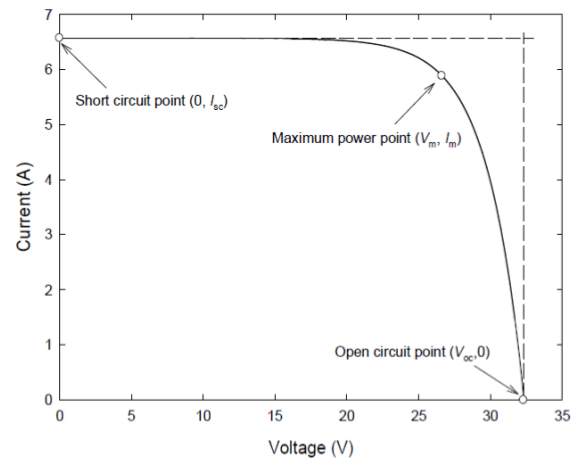
\includegraphics[width=0.90\textwidth]{ivcurve}
\centering
\caption{$ I-V $ characteristic curve of an ideal PV cell. Source: \cite{Saloux}.}
\label{fig:ivcurve}
\end{figure}

Hence, the short-circuit current, the open-circuit voltage, the maximum power voltage and current are written as defined by \cite{Saloux} and shown from Equations \ref{eq:Isc} to \ref{eq:Im}.

\begin{equation}
\label{eq:Isc}
I_{sc}=I_{ph}\vert_{V=0}
\end{equation}

\begin{equation}
\label{eq:Voc}
V_{oc}=\dfrac{aNk_{B}T}{q}ln\left( 1+\dfrac{I_{sc}}{I_{0}} \right) 
\end{equation}

\begin{equation}
\label{eq:exp}
exp\left( \dfrac{qV_{oc}}{aNk_{B}T} \right) = \left(1+\dfrac{qV_{m}}{aNk_{B}T} \right) exp \left( \dfrac{qV_{m}}{aNk_{B}T} \right) 
\end{equation}

\begin{equation}
\label{eq:Im}
I_{m} =I_{ph}-I_{0}\left[ exp \left( \dfrac{qV_{m}}{aNk_{B}T} \right) -1 \right] 
\end{equation}

Equation \ref{eq:exp} is not explicit with the PV key parameters, therefore need to be rewritten in a different way. A PV cell has a hybrid behavior, i.e., a current-source at the short-circuit point and voltage-source at the open-circuit point \cite{Saloux}. These two regions are characterized by two asymptotes of the $ I-V $ curve in Fig. \ref{fig:ivcurve}, where the transition is a compromise between both behaviors. It is interesting to observe that the maximum power point corresponds to a trade-off condition, where the current is still high enough before it starts decreasing with increasing the output voltage (Fig. \ref{fig:ivcurve}).

Based on this, the tangent of the I-V curve can be used to evaluate the transition between current- to voltage-source controlled regions; this operation yields Equation \ref{eq:didv}.

\begin{equation}
\label{eq:didv}
\dfrac{dI}{dV}=-\dfrac{qI_{0}}{aNk_{B}T}exp \left( \dfrac{qV}{aNk_{B}T}  \right) 
\end{equation}

The derivative of Equation \ref{eq:didv} is used to calculate the output voltage that corresponds to the maximum power operation condition of the cell. Therefore, the Equation \ref{eq:Vmderiv} is generated.

\begin{equation}
\label{eq:Vmderiv}
V_{m}=\dfrac{aNk_{B}T}{q} ln \left( -\dfrac{qNk_{B}T}{qI_{0}} \left( \dfrac{dI}{dV}  \right)_{V_{m}}   \right) 
\end{equation}

It is evident that Equation \ref{eq:Vmderiv} requires an expression of the derivative of the current with voltage evaluated at the maximum power point. The fact that the maximum power corresponds to an extreme, the variation of the maximum output power with voltage is relatively small, i.e., a change on $ V_{m} $ has a relatively small effect on the maximum power of the cell \cite{Saloux}. Consequently, considering the asymptotic behavior of the $I-V$ curve at short- and open-circuit conditions, the derivative required by Equation 10 can be calculated as shown in Equation \ref{eq:dIdV_Vm}.

\begin{equation}
\label{eq:dIdV_Vm}
\dfrac{dI}{dV}\vert_{V_{m}} \cong -\dfrac{0-I_{sc}}{V_{oc}-0}=\dfrac{I_{sc}}{V_{oc}}
\end{equation}

Replacing the Equation \ref{eq:dIdV_Vm} into Equations \ref{eq:Vmderiv} and \ref{eq:Im}, the voltage and the current at the maximum power point and consequently the maximum output power, are expressed by Equations \ref{eq:Vmfinal}, \ref{eq:Imfinal}, and \ref{eq:Pm} ($ P_{m}=V_{m}I_{m} $). These equations are used to calculate the key cell parameters at the maximum power point as function cell temperature and parameters from the manufacturer's data-sheet.

\begin{equation}
\label{eq:Vmfinal}
V_{m}=\dfrac{aNk_{B}T}{q} ln \left( \dfrac{aNk_{B}T}{qI_{0}} \dfrac{I_{sc}}{V_{oc}}  \right) 
\end{equation}

\begin{equation}
\label{eq:Imfinal}
I_{m} = I_{ph} + I_{0} - \dfrac{aNk_{B}T}{q} \left( \dfrac{I_{sc}}{V_{oc}} \right)  
\end{equation}

\begin{equation}
\label{eq:Pm}
P_{m} = \left[ \dfrac{aNk_{B}T}{q} ln \left( \dfrac{aNk_{B}T}{qI_{0}} \dfrac{I_{sc}}{V_{oc}}  \right) \right] \times \left[ I_{ph} + I_{0} - \dfrac{aNk_{B}T}{q} \left( \dfrac{I_{sc}}{V_{oc}} \right)  \right] 
\end{equation}


However, the photocurrent delivered by the constant current source ($ I_{ph} $) or even the reverse saturation current ($ I_{0} $) are not given by PV manufacturers. Therefore, Equation \ref{eq:Iph} is used to calculate the photocurrent as function of irradiance and temperature \cite{Villalva}.

\begin{equation}
\label{eq:Iph}
I_{ph}=\dfrac{G}{G_{ref}} \left[ I_{ph,ref} + \mu_{I} \left( T-T_{ref} \right)    \right] 
\end{equation}

Where the reference state (STC) of the cell is given by the solar irradiance $ G_{ref}=1000 W/m^{2} $, and the temperature $ T_{ref}=298.15 K (=25^{o}C) $.

In Equation \ref{eq:Iph}, $ \mu_{I} $ is the short-circuit current temperature coefficient ($A/K$) and corresponds to the photocurrent obtained from a given PV cell working at (STC or standard test conditions) reference conditions (provided by PV manufacturers). $ I_{ph,ref} $ can also be approximated to the reference short-circuit current that is provided by PV manufacturers ($ I_{sc,ref} $) as shown by \cite{Jakhrani}.

The cell temperature ($ T $) can be obtained from \cite{Ross} and is shown in Equation \ref{eq:Tcell}.

\begin{equation}
\label{eq:Tcell}
T = T_{air} + \dfrac{NOCT-20}{800}G
\end{equation}

Where $ T_{air} $ is the ambient temperature, $NOCT$ is the nominal operating cell temperature (in $^{o}$C) that is found at the PV manufacturer's data-sheet, and $G$ is the solar irradiance ($ W/m^{2} $) of the place where the PV system is deployed.

Furthermore, \cite{Villalva} have proposed a relationship, which allows the saturation current ($ I_{0} $) to be expressed as a function of the cell temperature. In this study, this relation is explicitly written based on cell open-circuit conditions using the short-circuit current temperature coefficient as well as the open-circuit voltage temperature coefficient (Equation \ref{eq:I0}).

\begin{equation}
\label{eq:I0}
I_{0} = \dfrac{I_{sc,ref} + \mu_{I}(T - T_{ref})}{exp \left[ \dfrac{q(V_{oc,ref} + \mu_{V} (T - T_{ref}))}{aNk_{B}T}    \right] -1}
\end{equation}

Where $ V_{oc,ref} $ is the reference open-circuit voltage, and $ \mu_{V} $ is an open-circuit voltage temperature coefficient ($ V/K $).

The ideality (or quality) factor of the diode $ a $, which is usually considered as a constant \cite{Villalva}, is determined in the reference state. Using the maximum power point current equation (Equation \ref{eq:Pm}) and the saturation current in the reference temperature given by Equation \ref{eq:I0}, the diode quality coefficient is determined by Equation \ref{eq:a}.

\begin{equation}
\label{eq:a}
a = \dfrac{q(V_{m,ref}-V_{oc,ref})}{Nk_{B}T} \dfrac{1}{ln \left( 1 - \dfrac{I_{m,ref}}{I_{sc,ref}}  \right) }
\end{equation}

Where $ V_{mref} $, $ V_{oc,ref} $, $ I_{m,ref} $, and $ I_{sc,ref} $ are key cell values obtained under both actual cell temperature and solar irradiance conditions, usually provided by manufacturers.

The model is now completely determined; it requires the actual cell temperature (or the air temperature), the actual solar irradiance and common data provided by manufacturers.

If the PV cells are in parallel, then there is a parallel array. Therefore, there will be a change at the $ I_{ph} $ and $ I_{0} $and the resulting current is given by Equation \ref{eq:Iarray}, as demonstrated in \cite{Saloux}.

\begin{equation}
\label{eq:Iarray}
I_{array} = (N_{cells in parallel})(I_{one cell})
\end{equation}

Where $ I_{one cell} $ is the current from Equation \ref{eq:Imfinal}.

In addition, if the panels are in series, the current do not change but the total voltage is the sum of the each panel's voltage.

\begin{equation}
\label{eq:Varray}
V_{array} = (N_{cells in series})(V_{one panel})
\end{equation}

Where $ V_{one panel} $ is the voltage from Equation \ref{eq:Vmfinal}.

Besides the model verification, there is the prior stage of project sizing check, which is simple, based on manufacturer's data and information from the sizing and the site. 

First is necessary to correct the energy consumption that was estimated to the load ($E_{consumption}$). That is done by Equation \ref{eq:Ecorrected}, according \cite{Pinho}. Where the efficiency of batteries ($\eta_{b}$), controller ($\eta_{c}$), and the inverter ($\eta_{i}$) are considered.

\begin{equation}
\label{eq:Ecorrected}
E_{corrected} = \dfrac{E_{consumption}}{ \eta_{b} \eta_{c} \eta_{i} }
\end{equation}

The total minimum number of solar panels necessary($ N_{TPmin} $) is calculated by Equation \ref{eq:NTPmin}, and the check is done with the Equation \ref{eq:NTP}, where the sized number of panels ($ N_{TP} $) must be greater than the result from Equation \ref{eq:NTPmin}.

\begin{equation}
\label{eq:NTPmin}
N_{TPmin} = \dfrac{E_{corrected}}{E_{p}}
\end{equation}

\begin{equation}
\label{eq:NTP}
N_{TP} \geq N_{TPmin}
\end{equation}

Particularly, the total number of panels is series ($ N_{PSmin} $) and parallel ($ N_{PPmin} $) are given by the Equations \ref{eq:NPSmin} and \ref{eq:NPPmin}, respectively. With the check did by Equations \ref{eq:NPS} and \ref{eq:NPP}. $ V_{system} $ is the DC voltage of the bus, and is a design decision (normally 12, 24 or 48 V).

\begin{equation}
\label{eq:NPSmin}
N_{PSmin} = \dfrac{V_{system}}{V_{m,ref}}
\end{equation}

\begin{equation}
\label{eq:NPPmin}
N_{PPmin} = \dfrac{N_{TPmin}}{N_{PSmin}}
\end{equation}

\begin{equation}
\label{eq:NPS}
N_{PS} \geq N_{PSmin}
\end{equation}

\begin{equation}
\label{eq:NPP}
N_{PP} \geq N_{PPmin}
\end{equation}


\subsubsection{The Battery Storage Model }
Because of the fluctuating nature of the output delivered by the PV arrays, batteries are necessary in a PV system. Thus, during the hours of sunshine, the PV system feeds directly the load and the excess electrical energy is stored in the battery. During the night, or during a period with low solar irradiation, energy is supplied to the load from the battery \cite{Mellit}.
  
Several models have been presented in the literature. However, regardless of the model, normally the following parameters are required: 

\begin{itemize}
\item Nominal capacity ($ q_{m} $), is the number of Ampère-hours ($ Ah $) that can maximally be extracted from the battery, under predetermined discharge conditions.
\item State of charge ($ SOC $), is the ratio between the present capacity and the nominal capacity, i.e., $ SOC = q/q_{max} $. Obviously $ 0<SOC<1 $. If $ SOC=1 $, then the battery is totally charged; and if $ SOC=0 $, the battery is fully discharged
\item Charge (or discharge) regime.This parameter reflects the relationship between the nominal capacity of a battery and the current at which it is charged (or discharged). It is expressed in hours: for instance, discharge regime is 30h for a battery of 150 Ah that is discharged at 5A.
\item Efficiency ($\eta_{b}$), is the ratio of the charge extracted during discharge divided by the amount of the charge needed to restore the initial state of charging or discharging current. 
\item Lifetime, is the number of charge/discharge cycles the battery can sustain before losing 20\% of its nominal capacity.
\end{itemize}

The merit of a stand-alone PV system is evaluated in terms of the reliability of the electricity supply to the load and in terms of the long-term efficiency of the components. The battery efficiency was described in this section, and the liability is quantified by the concept of loss of load probability (LLP). LLP is defined as the ratio between the Ampere-hour deficit and the Ampere-hour demand, both with respect to the load, over a long period of time \cite{Copetti}. 

In general, the battery models view the battery as a voltage source $ E $ in series with an internal resistance $ R_{0} $, as shown in Fig. \ref{fig:batteryckt}. 

\begin{figure}[h]
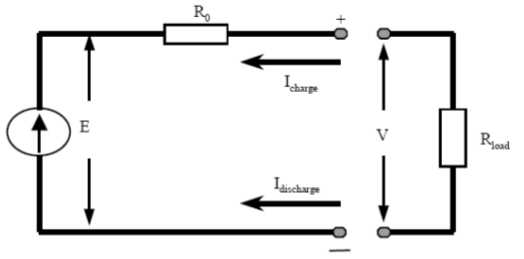
\includegraphics[width=0.7\textwidth]{batteryckt}
\centering
\caption{Schematic diagram of the battery. Source: \cite{Hansen}.}
\label{fig:batteryckt}
\end{figure}


The terminal voltage of the battery can be expressed in terms of its open circuit voltage and the voltage across the internal resistance of the battery \cite{Sukamongkol}, as shown by Equation 31.  

Where $ V_{b} $ is the battery terminal voltage, $ E_{oc} $ is the battery circuit voltage, $ I_{b} $ is the battery current, and $ R_{b} $ is the internal resistance of the battery.

The battery model, which describes the relationship between the voltage, current and the state of charge, can be found in \cite{Copetti}, \cite{Manwell93}, and \cite{Manwell94}.  

The Kinetic Battery Model (KiBaM) of Manwell and McGowen \cite{Manwell93} was developed at the University of Massachusetts to predict the performance of the battery, based on manufacturer's data. However, it uses some data extracted from tested batteries in laboratory. Therefore is not suitable to this study. 

Most of the created models were used to simulate and optimize PV storage system based on lead-acid batteries. That kind of battery is the most common used batteries in PV application, owing to their relative low cost and wide availability \cite{Copetti}. 

Here, the model adopted is the based on \cite{Copetti}, who uses manufacturer's data and allows finding relations among voltage, current, state of charge and temperature. 

The discharge voltage equation is shown in Equation \ref{eq:bat_Vd}. The first term represents the voltage variation with the state of charge ($ SOC $), i.e., the electrolyte concentration, and the second is the variation due to internal resistance variation.

\begin{equation}
\label{eq:bat_Vd}
V_{d} = \left[ 2.085-0.12(1-SOC) \right] - \dfrac{I}{C_{10}} \left( \dfrac{4}{1+I^{1.3}} + \dfrac{0.27}{SOC^{1.5}}+0.02 \right) (1-0.007 \Delta T)
\end{equation}

Where $ C_{10} $ means 10h of rated capacity, which is standard on the manufacturer's data-sheet, $ \Delta T $ is temperature variation ($ \Delta T=T-T_{ref} $, $ T_{ref}=25^{o}C $, $ SOC $ indicates how much electric charge is stored in the cell at given time, defined by Equation \ref{eq:SOCbat}.

\begin{equation}
\label{eq:SOCbat}
SOC = \left( 1 - \dfrac{Q}{C} \right) 
\end{equation}

Where $ Q $ is the charge delivered at the time of interest ($ Q=It $), and C is the battery capacity.

The ratio between $ Q $ and $ C $ represents the depth of discharge ($ DOD $) or the farction of discharge, i.e., $ DOC=1-SOC $.

The efficiency of the battery discharge is assumed to be 100\%, according \cite{Copetti}; however, the total amount of useful charge available during discharge is limited by the current rate and temperature given by Equation \ref{eq:CC10}. This equation, called of capacity, is normalized with respect to discharge current corresponding to $ C_{10} $ rated capacity ($ I_{10} $).

\begin{equation}
\label{eq:CC10}
\dfrac{C}{C_{10}} = \dfrac{1.67}{1+0.67 \left( \dfrac{I}{I_{10}} \right)^{0.9} }(1+0.005 \Delta T)
\end{equation}

Note that when the discharge current tends to zero at 25$^{o}$C, the maximum capacity that can be removed is about 67\% over the capacity.

For the charging process, however, the parameters are presented in Equation \ref{eq:Vcbat}.

\begin{equation}
\label{eq:Vcbat}
V_{c} = [2+0.16SOC]+ \dfrac{I}{C_{10}} \left( \dfrac{6}{1+I^{0.86}} + \dfrac{0.48}{(1-SOC)^{1.2}} + 0.036  \right) (1-0.025 \Delta T)
\end{equation}

SOC can be calculated easily at any point during the discharge period; however, during recharge it is much more difficult \cite{Copetti}.

Generally, the efficient region is where $ SOC $ is below $ 0.7 $ and $ V_{c} $ is less than $2.3 V$ per cell. The efficiency drops to zero at full charge and the function that represents the charge efficiency ($ \eta_{c} $) variation with state of charge and current rate is given in Equation \ref{eq:efficcharge}.

\begin{equation}
\label{eq:efficcharge}
\eta_{c} = 1 - exp \left[ \dfrac{20.73}{\dfrac{I}{I_{10}}+0.55} (SOC-1) \right] 
\end{equation}

\cite{Copetti} show that, during overcharge, gassing occur and tests demonstrated that the final charge voltage ($ V_{ec} $) increases with the current intensity and with the decreasing of the temperature (Equation \ref{eq:Vec}). It was created a function for the gassing voltage as well, as shown in Equation \ref{eq:Vg}. In addition, the overcharge phenomenon can be represented by Equation \ref{eq:Voverc}.

\begin{equation}
\label{eq:Vec}
V_{ec} = \left[ 2.45 + 2.011 ln \left( 1+\dfrac{I}{C_{10}} \right)  \right] (1-0.002 \Delta T)
\end{equation}

\begin{equation}
\label{eq:Vg}
V_{g} = \left[ 2.24 + 1.97 ln \left( 1+\dfrac{I}{C_{10}} \right)  \right] (1-0.002 \Delta T)
\end{equation}

\begin{equation}
\label{eq:Voverc}
V_{c} = V_{g} + (V_{ec} - V_{g}) \left[ 1- exp \left( \dfrac{Ah_{restored}-0.95C}{I\tau}  \right)    \right] 
\end{equation}

Where $ Ah_{restored} $ represents the Ampère-hour stored in the battery with regard to the battery capacity ($ C $) during this hour.

The function assumes that 95\% of the capacity was already restored at the start of overcharge.

The time constant of the phenomenon ($ \tau $) is reversely proportional to the charge intensity and can be written by Equation \ref{eq:tau}.

\begin{equation}
\label{eq:tau}
\tau = \dfrac{17.3}{1+852 \left( \dfrac{I}{C_{10}} \right) ^{1.67} }
\end{equation}

Therefore, to model the voltage ($ V_{c} $) evolution of the battery, equation \ref{eq:Vcbat} can be used up the start of gassing ($ V_{c} \leq V_{g} $). And during overcharging ($ V_{c} > V_{g} $), Equation \ref{eq:Voverc} can be used until a constant final voltage ($ V_{ec} $) is reached.

The storage capacity of the battery can be calculated using Equation \ref{eq:stor}, as defined in \cite{Wenham}.

\begin{equation}
\label{eq:stor}
Storage capacity = \dfrac{N_{C}E_{load}}{DOD \eta _{b}}
\end{equation}

Where $ DOD $ is the maximum possible depth of battery discharge, $ E_{load} $ is the average energy consumed by the load, $ N_{C} $ is the largest number of continuous cloudy days of the area, and $ \eta_{b} $ is the efficiency of the battery.

As an example of this formula application, as shown by \cite{Abdulateef}, considering that an off-grid PV system is intended to supply $1.5 kW/48 V$ for 24 hours ($=36 kWh$); The largest number of continuous cloudy days in the selected site is about 1 day; For a maximum depth of discharge for the battery $DOD$ of $0.8$ and battery efficiency $80\%$.

Then the storage capacity using Equation \ref{eq:stor} becomes $56.3 kWh$. Since the selected DC bus voltage is $48 V$, then the required Ampere-hours of the battery is $1173 Ah$ ($56.3 kWh/48$). If a single battery of 12 V and 350 Ah is considered, then four batteries are connected in series ($4 \times 350 Ah = 1400 Ah$).

At this research, it was considered a simplified model for charging (Equation \ref{eq:charge}) and discharging (Equation \ref{eq:discharge}) of the batteries, even considering that the process is not linear and depends on the temperature. The equations are used to update the $SOC$ of the batteries, and have the number of hours ($ Num_{h} $) as a variable. There is a factor (1.15) which is present at the charging equation, and is necessary to express that during the charging process is usual to reach 115\% of the battery capacity

\begin{equation}
\label{eq:charge}
SOC_{charge} = SOC_{previous} + \dfrac{100*Pm*Num_{h}}{V_{system}*capacity*N_{BP}*1.15}
\end{equation}

\begin{equation}
\label{eq:discharge}
SOC_{discharge} = SOC_{previous} - \dfrac{100*I_{drained}*Num_{h}}{capacity}
\end{equation}


Besides the model verification, there is also the prior stage of project sizing check, as did to the solar panel. First is necessary to define the total capacity of the battery bank, as shown by Equation \ref{eq:Cbank}.

\begin{equation}
\label{eq:Cbank}
C_{bank} = \dfrac{E_{corrected} \times autonomy}{V_{system} \times DOD}
\end{equation}

The variable $ autonomy $ is a design definition and normally has a value ranging from 6 to 48h. The other variables were discussed previously.

Following, is done the total (minimum) number of batteries, as show by Equation \ref{eq:Nbtotal}. Moreover, the Equation \ref{eq:batcheck} perform the final sizing check, considering the number of batteries in series ($ N_{BS} $) and the number of batteries in parallel ($ N_{BP} $) that were established to the project.

\begin{equation}
\label{eq:Nbtotal}
N_{B}total = N_{BS}min \times N_{BP}min = \dfrac{V_{system}}{V_{bat}} \times \dfrac{C_{bank}}{C_{20}}
\end{equation}

\begin{equation}
\label{eq:batcheck}
\left( N_{BS} \times  N_{BP} \right) \geq N_{B}total
\end{equation}

\subsubsection{Controller Model}
Depending on the literature, the controller can receive different names: controller \cite{Hansen}, charge controller \cite{Mahanta} and \cite{Chauhan}, regulator \cite{Mellit}, DC-DC converter with MPPT and switch \cite{Dhanowa}, \cite{Yatimi}, \cite{Abdulateef}, \cite{Roy}. However, in this study, in order to simplify, the term used is controller. 

The controller is a set of items (DC-DC converter, a MPPT and switches) and can be defined as the responsible to manage the energy flow to PV system, batteries and loads by collecting information on the battery voltage and knowing the maximum and minimum values acceptable for the battery voltage. According to \cite{Pinho}, controllers aim to protect the battery (or batteries) against the excessive charge and discharge, improving its lifetime. 

As defined by \cite{Hansen} and \cite{Mellit}, all power systems must include a control strategy, which describes the interactions between its components. The use of battery as a storage form implies thus the presence of a charge controller. 

In general, there are two main operating modes for the controller: normal operating condition, when the battery voltage fluctuates between maximum and minimum voltages; and overcharge or over-discharge conditions, which occur when the battery voltage reaches some critical values. 

In \cite{Mellit} was established that the controller allows the management of energy between the load and the battery. The input signals for regulator model are the battery current ($ I_{br} $), PV generator's voltage ($ V_{PV} $), PV generator's current ($ I_{PV} $), and battery voltage ($ V_{b} $). The outputs are battery ($ I_{rb} $) current and used current ($ I_{u} $). 

According \cite{Hansen}, to protect the battery against an excessive charge, the PV arrays are disconnected from the system, when the terminal voltage increases above a certain threshold $ V_{max \textunderscore off} $ and when the current required by the load is less than the current delivered by the PV arrays. PV arrays are connected again when the terminal voltage decreases below a certain value $ V_{max \textunderscore on} $. This can be done by using a switch with a hysteresis cycle, as illustrated in Fig. \ref{fig:controllerover}. 

\begin{figure}[h]
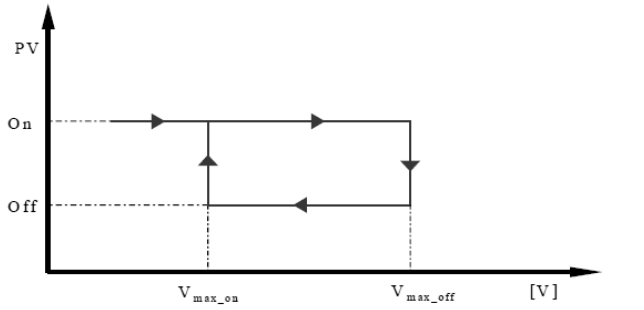
\includegraphics[width=0.7\textwidth]{controllerover}
\centering
\caption{Operating principle of an overcharge protector. Source: \cite{Hansen}.}
\label{fig:controllerover}
\end{figure}

To protect the battery against excessive discharge, the load is disconnected when the terminal voltage falls below a certain threshold i and when the current required by the load is larger than the current delivered by the PV arrays \cite{Hansen}. The load is reconnected to the system, when the terminal voltage is above a certain value i, using a switch with a hysteresis cycle, as shown in Fig. \ref{fig:controllerdisc}. 

\begin{figure}[h]
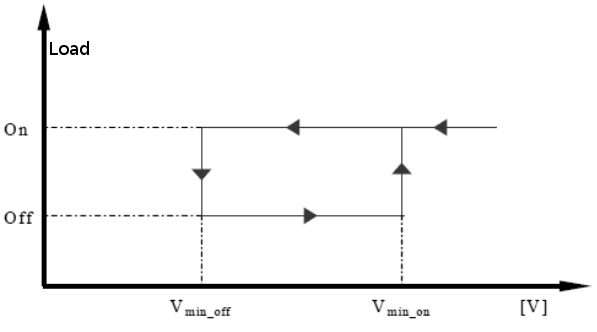
\includegraphics[width=0.7\textwidth]{controllerdisc}
\centering
\caption{Operating principle of a discharge protector. Source: \cite{Hansen}.}
\label{fig:controllerdisc}
\end{figure}

According to \cite{Lorenzo}, the switches may either be electromechanical (relay, contactors, etc.) or solid state (bipolar transistors, MOSFET's, etc.). 

The steps in the modeling of the controller process are summarized in Table \ref{table:controller}.

\begin{table}[!t]
%% increase table row spacing, adjust to taste
\renewcommand{\arraystretch}{1.3}
% if using array.sty, it might be a good idea to tweak the value of
% \extrarowheight as needed to properly center the text within the cells
\caption{Summary of the controller process. Source: \cite{Hansen}.}
\label{table:controller}
\centering
%% Some packages, such as MDW tools, offer better commands for making tables
%% than the plain LaTeX2e tabular which is used here.
\begin{tabular}{c | c | c }
\hline
\hline
Step  & Constraint & Command\\
\hline
\hline
(1) & \makecell{If $V > V_{max \textunderscore off}$ and $I_{load} < I_{pv}$} & \makecell{Disconnect PV array from the system}\\
\hline
(2) & \makecell{If command (1) is done and $V < V_{max \textunderscore on}$} & \makecell{Reconnect PV array to the system}\\
\hline
(3) & \makecell{If $V < V_{min \textunderscore off}$ and $I_{load} > I_{pv}$} & \makecell{Disconnect the load from the system}\\
\hline
(4) & \makecell{If command (3) is done and $V > V_{min \textunderscore on}$} & \makecell{Reconnect the load to the system}\\
\hline
\hline
\end{tabular}
\end{table}

Regarding the DC-DC converter, the most basic idea is that the power is converted while altering the current and voltage. 

As shown in \cite{Abdulateef}, the DC-DC converter is used to increase the efficiency of the PV system by matching the voltage generated by PV array to the voltage required by the load. The output power ($ P_{out} $) of DC-DC converter is given by Equation \ref{eq:poutcont}. 

\begin{equation}
\label{eq:poutcont}
P_{in = P_{out}}
\end{equation}

Assuming that the efficiency of the controller ($ \eta_{c} $) is a manufacturer's data, from Equation \ref{eq:poutcont} is possible to reach Equation \ref{eq:potcont}.

\begin{equation}
\label{eq:potcont}
V_{in} I_{in} \eta_{c} = V_{out} I_{out}
\end{equation}

Where $ V_{in} $ is the voltage across the PV array, $ I_{in} $ is the current output of PV array, $ V_{out}=V_{b}=V_{system} $ is the  DC bus voltage, and $-I_{out}$ is the output current from the converter, when all the other values are known.

The output voltage is related to the input voltage as a function of duty cycle of the switch (\cite{Abdulateef}). 
 
A DC-DC converter can either be step-up (Boost), step-down (Buck), or both increase and decrease (Buck-Boost) the voltage, as defined by \cite{Mahanta}. In addition, there is the Cuk converter, which is a Buck-Boost converter with an inverting topology \cite{Catherine}. 

For the Cuk converter, the relationship is expressed by \ref{eq:voutvin} as show in \cite{Abdulateef}.

\begin{equation}
\label{eq:voutvin}
\dfrac{V_{out}}{V_{in}} = \dfrac{D}{D-1}
\end{equation}

Where $D$ is the duty cycle or ratio of the circuit converter, i.e., it is defined as the ratio of the on time of the switch to the total switching period.
 
The DC/DC converter should always operate in the MPPT to maximize the PV array efficiency and consequently increase the efficiency of the PV system, as defined in \cite{Yatimi}.
  
Various types of MPPT schemes are proposed by researchers, namely open circuit, short circuit, perturb and observe (P\& O)/hill climbing, incremental conductance, and so forth, as shown by \cite{Haque}.
 
As the MPPT definition and the equations to get the maximum power from the PV panels was described at the end of the PV panel modeling, the important here is to notice that the Equation \ref{eq:voutvin} defines the relationship between the input signal, the efficiency of the controller and the output power.
 
One more time, some steps must be done to check the sizing project of the controller, prior the verification phase. Initially the controller must meet the voltage requirement of the PV system, as shown by Equation \ref{eq:vcvsystem}. 

\begin{equation}
\label{eq:vcvsystem}
V_{c} = V_{system}
\end{equation}

Following, the short circuit reference information from the manufacturer's solar panel must be corrected to the cell temperature, as shown by Equation \ref{eq:iscamb}.

\begin{equation}
\label{eq:iscamb}
I_{sc,amb} = I_{sc,ref} \times \left[ 1 + \eta_{I} \times (T-25) \right] 
\end{equation}

The controller must meet the maximum current from the PV array (Equations \ref{eq:icmin} and \ref{eq:icicmin}).

\begin{equation}
\label{eq:icmin}
I_{c,min} = I_{sc,amb} \times N_{PP}
\end{equation}

\begin{equation}
\label{eq:icicmin}
I_{c} \geq I_{c,min}
\end{equation}

The number of controllers required for the off-grid PV system, as defined by \cite{Yatimi}, is calculated using Equation \ref{eq:numberofcmin}. In addition, the final sizing check is did by Equation \ref{eq:numberofc}, who validate the number of controllers adopted.

\begin{equation}
\label{eq:numberofcmin}
number_{controllers} = \dfrac{Total \, max \, power \, of \, PV}{Controller \, max \, power} =  \dfrac{P_{m,ref} \times N_{TP}}{V_{system} \times I_{controller,max}}
\end{equation}

\begin{equation}
\label{eq:numberofc}
N_{controller} \geq number_{controllers}
\end{equation}

\subsubsection{The inverter model}
As shown by \cite{Mellit}, the PV arrays produce DC and therefore when the PV system contains an AC load, a DC/AC conversion is required. An inverter is a converter, where the power flows from DC to AC side, i.e., having a DC voltage as input; it produces AC voltage, as output. The role of the inverter is to keep the voltage constant on the AC side, i.e., at the rated voltage (127 V or 220 V, for example), and to convert the input power $ P_{in} $ into the output power $ P_{out} $ with the best possible efficiency \cite{Hansen}.

The inverter is characterized by a power dependent efficiency $ \eta_{i} $ given by \cite{Hansen} as shown by Equation \ref{eq:efficinv}.

\begin{equation}
\label{eq:efficinv}
\eta_{i} = \dfrac{P_{out}}{P_{in}} = \dfrac{V_{AC} I_{AC} cos\varphi}{V_{DC}I_{DC}}
\end{equation}

Where $ I_{DC} $ is the current required by the inverter from the DC source in order to be able to keep the rated voltage on the AC side, $ V_{DC} $ is the input voltage to the inverter delivered by the DC source (PV panel or battery),  $ V_{AC}  $ and $ I_{AC} $ are the output voltage and current, respectively, and $ cos \varphi $ can be found from the inverter's data-sheet.

Therefore, with this equation it is possible to simulate the output power of the inverter, based on information from the inverter's data-sheet and from the DC module or the PV panel that feed the inverter (which are obtained by this study model). 

The sizing project check of the inverter is done through three Equations. Equation \ref{eq:vindc} ensure that the input voltage of the controller meet the voltage of the system. Equation \ref{eq:voutac} ensures that the output voltage of the controller meet the AC voltage of the load. Moreover, Equation \ref{eq:invcheck} ensures that the controller can support the total demand of the load and the surge power.

\begin{equation}
\label{eq:vindc} 
V_{in}DC = V_{system}
\end{equation}

\begin{equation}
\label{eq:voutac} 
V_{out}AC = V_{AC}
\end{equation}

\begin{equation}
\label{eq:invcheck} 
\left[ (Demand \leq P_{AC,ref}) \, and \, (P_{surge} \leq MAX_{AC,ref}) \right] 
\end{equation}


///////begin-verification 
\subsection{Sizing and Simulation of Stand-alone Solar PV systems}
The sizing and validation of a PV system can be done by hand or with the aid of tools. Here we reference the critical period~\cite{Pinho} as an effective method to stand-alone PV sizing.
%
%In order to address different aspects of the PV system design, there are various software tools available in the literature~\cite{Rajanna,Rawat}.
%public domain and commercial software available for the PV market. 
%According to \cite{Brooks}, t
%%%%%%%%%%The capabilities of tools available in the literature range from simple solar resource and energy production estimation, %to site survey and system design tools,
% to complex financial analysis and project optimization. 
%Some tools also provide support to rebate programs applications and tax incentives (specific to each country or region), while other programs and worksheets focus on the technical aspects of system sizing and design.
%
%Manufacturers and integrators have yet their proprietary software to perform inverter string sizing and various system sizing and design tools, with the drawback to just include their own products among the possibilities of choice. 

The most popular softwares are summarized at Table~\ref{table:softwares}: PVWatts, SAM, HOMER, RETScreen, and Hybrid2~\cite{Pradhan,Swarnkar,NRELDobos,NRELBlair,Mills}.
%\subsection{PVWatts Calculator}
%According to \cite{Freeman} and \cite{NRELDobos}, it is a web application developed by the National Renewable Energy Laboratory (NREL), which estimates the electricity production of a grid-connected roof- or ground-mounted photovoltaic system based on a few inputs. According to \cite{NRELDobos}, to use the calculator, it is necessary to provide information about the system's location, basic design parameters, and system economics. PVWatts calculates estimated values for the system's annual and monthly electricity production, and for the electricity monetary value. This tool is suitable for very preliminary studies of a potential location for a photovoltaic system that uses crystalline silicon or thin film photovoltaic modules. The production estimates that PVWatts computation do not account for many factors that are important in the design of a photovoltaic system, therefore it is necessary support of an energy expert. The calculator estimates the monthly and annual electricity production of a photovoltaic system using an hour-by-hour simulation over a period of one year. To represent the system's physical characteristics, PVWatts requires values for six inputs: System DC size; Module type; Array type; System losses; Array tilt angle; Array azimuth angle.
%
%\subsection{SAM}
%SAM or System Advisor Model is a software from the U.S. Department of Energy and National Renewable Energy Laboratory. According to \cite{NRELBlair} and \cite{Cameron2008}, SAM is intended to help users to determine whether the model meets their project constraints/specifications, and (also) to provide information for readers who do not plan to use the model, but want to learn about its capabilities. SAM is a performance and financial model designed to facilitate decision making for people involved in the renewable energy industry: Project managers and engineers; Financial and policy analysts; Technology developers; and Researchers. SAM makes performance predictions and cost of energy estimates for grid-connected power projects based on installation and operating costs and system design parameters that you specify as inputs to the model. Projects can be either on the customer side of the utility meter, where they buy and sell electricity at retail rates, or on the utility side of the meter, where they sell electricity at a price negotiated through a power purchase agreement. SAM is an electric power generation model and assumes that the renewable energy system delivers power either to an electric grid, or to a grid-connected building or facility to meet electric load. It does not model thermal energy systems that meet a thermal process load. As mentioned in \cite{NRELBlair}, SAM does not model isolated or off-grid power systems, and does not model systems with electricity storage batteries.
%
%\subsection{HOMER}
%As defined in \cite{HOMER}, actually is a set of two tools: HOMER Legacy and HOMER Pro. HOMER is an acronym for Hybrid Optimization Model for Multiple Energy Resources. HOMER Legacy is the original HOMER software version created at the National Renewable Energy Laboratory (NREL). HOMER Legacy is a free computer model that simplifies the task of evaluating design options for both off-grid and grid-connected power systems for remote, stand-alone, and distributed generation applications. HOMER's optimization and sensitivity analysis algorithms allow the user to evaluate the economic and technical feasibility of a large number of technology options. Since 2016 HOMER Legacy can be found at HOMER web site, but only available for students and nonprofit organizations, as defined in \cite{HOMER}, and has not support available. At the short-time only the commercial version will remain.
%
%The commercial version (paid), called HOMER Pro, as defined in \cite{Swarnkar}, is a tool for optimizing micro-grid design in all sectors, from village power and island utilities to grid-connected campuses and military bases. HOMER Pro put together three tools in one product: optimization, simulation, and sensitivity analysis. HOMER Pro provides the detailed rigor of chronological simulation and optimization in a model that is intended to be easy to use. It is adaptable to a wide variety of projects. For a village or community-scale power system, HOMER can model both the technical and economic factors involved in the project. For larger systems, HOMER can provide an overview that compares the cost and feasibility of different configurations. Chronological simulation is essential for modeling variable resources, such as solar and wind power and for combined heat and power applications, where the thermal load is variable. HOMER's sensitivity analysis helps determine the potential impact of uncertain factors such as fuel prices or wind speed on a given system. 
%
%\subsection{RETScreen}
%As mentioned in \cite{Pradhan}, RETScreen is a decision-support tool designed to help decision makers and energy professionals to evaluate the financial viability of renewable energy, energy efficiency, and/or co-generation projects.
%
%RETScreen models various types of renewable energy technologies (RETs), allowing for comparisons between technology options. The software can be used to evaluate benefits from both clean energy production from power generation projects and savings through energy efficiency projects, accounting for project costs, greenhouse gas emission reductions, and financial risk. The software is freely distributed (but with restrictions to save work or print), and had three different versions:
%
%\begin{itemize}
%\item RETScreen 4 (discontinued, requires Microsoft Excel to run); 
%\item RETScreen Software Suit, which includes the RETScreen 4 and a Windows-based graphical software that allows project owners to verify the ongoing energy performance of their facilities (discontinued in 2013);
%\item And the actual (2016) RETScreen Expert, which allows users to evaluate energy investments over an entire project life-cycle (including benchmarking, feasibility, and performance analysis) in a fully integrated way, and within one software platform. However, this version works is only Windows-based. This version has a complete paid version, in an annual subscription way.
%\end{itemize}
%
%As described by \cite{Pradhan}, RETScreen performs a five-step standard analysis: setting and site conditions; energy model; cost analysis; emission analysis, financial analysis, sensitivity, and risk analysis. It is developed and maintained by the Government of Canada, through the CanmetENERGY Varennes Research Centre of Natural Resources; in collaboration with: NASA; Renewable Energy and Energy Efficiency Partnership (REEEP); United Nations Environment Programme (UNEP), and the Global Environment Facility (GEF). RETScreen is available in 36 languages; it is a multi-awarded tool, and includes equipment databases for components manufactured and available worldwide.
%
%\subsection{Hybrid2}
%The Hybrid2 software package, as described in \cite{Mills}, is a user-friendly tool to perform detailed long-term performance and economic analysis on a wide variety of hybrid power systems. Hybrid2 is a probabilistic/time series computer model, using time series data for loads, wind speed, solar insolation, and temperature; and the power system is designed or selected by the user, in order to predict the performance of the hybrid power system. Variations in wind speed and in load within each time step are factored into the performance predictions. The code does not consider short-term system fluctuations caused by system dynamics or component transients. This program is not supported anymore and according to \cite{UMASS}, probably after the user performs the free download of the tool, it will not work on Windows platforms later than Windows XP, what is a limitation.
%
%Table~\ref{table:softwares} summarizes the off-the-shelf tools employed here, where 
As highlights, only HOMER and Hybrid2 perform off-grid system with battery backup analysis. %all the tools perform solar photovoltaic analysis; 
Additionally, HOMER and RETScreen include economical analysis or even optimization-sensitive analysis. However, commercial version of those tools, called RETScreen Expert and HOMER Pro, are available only for Microsoft Windows and the annual subscription typically range from US\$504.00 to US\$657.00.
%
\begin{table}[!t]
%% increase table row spacing, adjust to taste
\renewcommand{\arraystretch}{1.3}
% if using array.sty, it might be a good idea to tweak the value of
% \extrarowheight as needed to properly center the text within the cells
\caption{Comparative coverage of reference simulation software}
\label{table:softwares}
\centering
%% Some packages, such as MDW tools, offer better commands for making tables
%% than the plain LaTeX2e tabular which is used here.
\begin{tabular}{c | c | c | c | c | c}
\hline
\hline
Characteristic  & \rotatebox{90}{PVWatts} & \rotatebox{90}{SAM} & \rotatebox{90}{HOMER} & \rotatebox{90}{RETScreen} & \rotatebox{90}{Hybrid2}\\
\hline
\hline
Support & X & X & X & X &  \\
\hline
Off-grid systems &   &   & X & X & X\\
\hline
Hybrid systems &  &  & X & X & X\\
\hline
Photovoltaics & X & X & X & X & X\\
\hline
Batteries &  &  & X &  & X\\
\hline
\makecell{Main technical (T) \\ or economical(E)} & T & T & E & E & T \\
\hline
Optimization &  &  & X & X &  \\
\hline
Sensitive analysis &  &  & X & X & \\
\hline
\hline
\end{tabular}
\end{table}
%
%-------------------------------------------------------------------
%\subsection{Paper Proposal x Reference Tools}
%-------------------------------------------------------------------
%
In this study, HOMER was chosen to comparative with our proposed verification approach (Section~\ref{sec:results_indeed}).%All tools need some parameters inherently from manufacturer's catalog.
%, so the project starts with manufacturers and integrators tool to define the basic items of the project: panels, inverters, controllers, and batteries. 
%After that, the potential solution is analyzed in another tool to simulate or even optimize the proposed solution. Therefore, that is 
%Thus, the main challenge here is to demonstrate the application of software model checking to formally verify a stand-alone PV solution, thus proving that this approach is more effective and complete than other state-of-the-art tool such as HOMER Pro. The comparative evaluation between HOMER Pro and our approach is presented in Section~\ref{sec:results_indeed}.
%
%-------------------------------------------------------------------
\subsection{Component models for a stand-alone PV system }
%-------------------------------------------------------------------
%The main purpose of this section is to describe the models for the elements of a stand-alone PV system: PV generator, battery, controller, inverter, and load. 
%The mathematical modeling of the PV system is based on modular blocks, as illustrated in Fig.\ref{fig:blockdiagram}. It identifies the PV generator, batteries, charge controller, inverter, and AC load. 
A stand-alone PV system is illustrated in Fig.\ref{fig:blockdiagram}. The PV generator is a semiconductor device that can convert solar energy into DC electricity. %In Fig.\ref{fig:blockdiagram}, there are two variables that depend on the site where the system is deployed and the weather (i.e., solar irradiance $G$ and temperature $T$). 
For night hours or rainy days, power stored in batteries can be used and it implies the presence of a charge controller~\cite{Hansen}. The PV arrays produce DC and therefore when the PV system contains an AC load, a DC/AC conversion is required (inverter). The AC load dictates the behavior of AC electrical load from the house that will be fed by the system.
%
%The modular structure facilitates the modeling of the other system structures and replacement of elements, such as a DC load instead of an AC load. 
%
\begin{figure}[h]
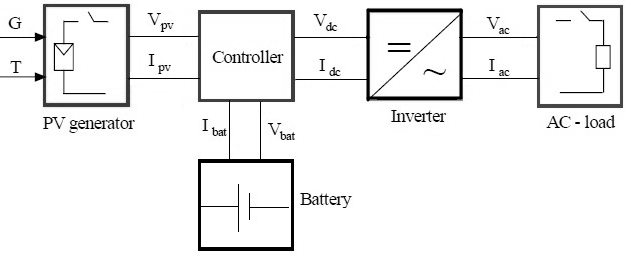
\includegraphics[width=0.80\textwidth]{blockdiagramPVS2}
\centering
\caption{Block diagram for a typical stand-alone PV system (adapted from~\cite{Hansen}).}
\label{fig:blockdiagram}
\end{figure}
%
%In the literature, there are several mathematical models available for each component of PV systems. At the next section, the mathematical model for each component is presented. 
%-------------------------------------------------------------------
\subsection{PV System Model}
\label{sec:PVsystemmodel}
%-------------------------------------------------------------------
%A photovoltaic PV generator is the whole assembly of solar cells, connections, protective parts, and supports. 
%In the present modeling, the focus is only on cell/module/array.
%
%%%%%%The basic element of a PV system is a PV cell, also called a solar cell. A solar cell is a semiconductor device that can convert solar energy into DC electricity. 
%The semiconductor materials (usually silicon), which are specially treated to form an electric field, positive on one side (backside) and negative on the other (towards the sun). When solar energy (photons) hits the solar cell, electrons are knocked loose from the atoms in the semiconductor material, creating electron-hole pairs \cite{Lorenzo}. If electrical conductors are attached to the positive and negative sides, forming an electrical circuit, the electrons are captured in the form of electric current $ I_{ph} $ (photocurrent).
%%%%%To increase their utility, a number of individual PV cells are interconnected together in a %sealed, weatherproof 
%%%%%package called panel or module. 
%For instance, a 12 V Panel will have 36 cells connected in series and a 24 V Panel will have 72 PV cells connected in series. In addition, to achieve the desired voltage and current, modules are wired in series and parallel into what is called a PV Array, as shown in Fig.\ref{fig:celmodarray}. The flexibility of the modular PV system allows designers to create PV systems that can meet a wide variety of electrical demands. 
%
%\begin{figure}[h]
%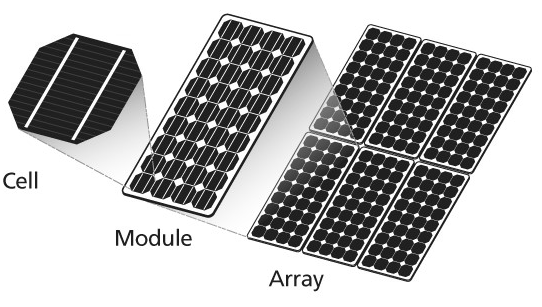
\includegraphics[width=0.4\textwidth]{celmodarray}
%\centering
%\caption{PV cell, module and array (Source: \cite{SamlexSolar})}
%\label{fig:celmodarray}
%\end{figure}
%
%%%%%The PV modules are generally rated under standard test conditions (STC), and the parameters required for the input of the PV modules are relying on meteorological conditions.
%the meteorological conditions of the area to be serviced by PV solution. %However, the climatic conditions are unpredictable due to the random nature of their occurrence \cite{Jakhrani}.
%, which leads to the following specification by the manufacturers:  solar radiation of 1000 W/m$^{2}$, cell temperature of 25$^{o}$C, and solar spectrum of 1.5. The parameters required for the input of the PV modules are relying on the meteorological conditions of the area to be serviced by photovoltaic solution. However, the climatic conditions are unpredictable due to the random nature of their occurrence \cite{Jakhrani}.
%
%These uncertainties lead to either over- or underestimation of energy yield from PV modules. An overestimation up to 40\% was reported as compared to the rated power output of PV modules \cite{Durisch}. The growing demand of photovoltaics technologies led to research in the various aspects of its components from cell technology to the modeling, size optimization, and system performance \cite{Yatimi}, \cite{Saloux}, \cite{Mellit}. 
%
%Modeling PV modules is one of the major components responsible for proper functioning of PV systems. However, the estimation of models is affected by various intrinsic and extrinsic factors, which ultimately influence the behavior of current and voltage. Therefore, perfect modeling is essential to estimate the performance of PV modules in different environmental conditions \cite{Jakhrani}.
% 
%Modeling provides the ways to understand the current, voltage, and power relationships of PV systems.
Mathematical models are required in order to allow the formal specification of the PV system. At this section we will summarize the models adopted at the paper.

\textbf{PV modules}: a wide variety of models exists. % for estimation of its power output  (and $I-V$ or $P-V$ curves). 
However, the present work will rely on the simplified model of 1-diode, illustrated in Fig. \ref{fig:equivckt}. This model has a small error rate, between 0.03\% and 4.68\% from selected PV panels tested~\cite{Saloux}.

%The performance of PV systems %, %that is, the output current/voltage curve ($I-V$ curve), 
%is usually studied using an equivalent circuit model~\cite{Yatimi}, which consists of a current source with one or two diodes connected in parallel, and up to two resistors, one connected in parallel and the other one in series, to take into account energy losses in this model~\cite{Cubas}. 
%Based on these electronic components, four basic configurations are normally used when studying photovoltaic systems, as shown by Fig. \ref{fig:equivckt}. 
\begin{figure}[h]
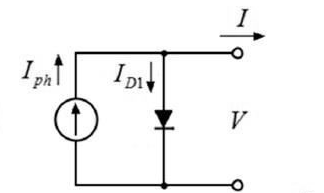
\includegraphics[width=0.40\textwidth]{equivckt1D}
\centering
\caption{1-diode equivalent PV cell/panel circuit model (adapted from~\cite{Cubas}).}
%\caption{Four different equivalent circuit models: (a) 1-diode; (b) 1-diode/1-resistor; (c) 1-diode/2-resistor; (d) 2-diode/2-resistor (Source: \cite{Cubas})}
\label{fig:equivckt}
\end{figure}

The Eq. \eqref{eq:1diodemodel} relates the output current, $I$, to the output voltage, $V$. %This model has a small error rate, between 0.03\% and 4.68\% from selected PV panels tested~\cite{Saloux}. %In addition, this mathematical modeling has the advantage of being an explicit model, which does not use iterative numerical calculation, which is time-consuming to computing~\cite{Cubas}.
\begin{equation}
\label{eq:1diodemodel}
I = I_{ph}-I_{D1}=I_{ph}-I_{0}\left[ exp \left( \dfrac{V}{NaV_{T}} \right)  \right], 
\end{equation}

\noindent where $I_{ph}$ is the photocurrent delivered by the constant current source; $I_{0}$ is the reverse saturation current corresponding to the diode; $N$ is the number of series-connected cells; %($N=1$ in a single cell configuration); 
$a$ is the ideality or quality factor ($a=1$ for ideal diodes and between $1$ and $2$ for real diodes); $V_{T}$ is the thermal voltage ($ V_{T}=k_{B}T/q $); $ k_{B} $ is the Boltzmann constant ($ 1.3806503\times10^{-23}\:J/K $); $T$ the temperature of cell in Kelvin; $q$ is absolute value of the electron's charge ($ -1.60217646\times10^{-19}\:C $).

%\begin{itemize}
%\item $I_{ph}$ is the photocurrent delivered by the constant current source; 
%\item $ I_{0} $ is the reverse saturation current corresponding to the diode; 
%\item $ N $ is the number of series-connected cells in the photovoltaic system to be analyzed; $ N=1 $ in a single cell configuration.
%	\begin{itemize}
%	\item $ N=1 $ in a single cell configuration. 	
%	\end{itemize}	  
%\item $ a $ is the ideality factor (or quality factor) that takes into account the deviation of the diodes from the Shockley diffusion theory; $a=1$ for ideal diodes and between $ 1 $ and $ 2 $ for real diodes.
%	\begin{itemize}
%	\item $a=1$ for ideal diodes and between $ 1 $ and $ 2 $ for real diodes. 	
%	\end{itemize}
%\item $V_{T}$ is the thermal voltage ($ V_{T}=k_{B}T/q $);
%	\begin{itemize}
%	\item $ k_{B} $ is the Boltzmann constant ($ 1.3806503\times10^{-23}J $); 
%	\item $ T $ the temperature of the p-n junction (or cell temperature) expressed in Kelvin; 
%	\item $ q $ is absolute value of the electron's charge ($ -1.60217646\times10^{-19}C $).	
%	\end{itemize}	 
%\end{itemize}
%
%This model has only three unknown parameters ($ I_{ph}$, $I_{0}$, and $a $), and it assumes that the series resistance is $ zero $ and shunt resistance is $ infinite $ and, thus, both of these parameters are ignored.
%
%The 1-diode/1-resistor model, is described by Equation \ref{eq:1d1rmodel}. 
%
%\begin{equation}
%\label{eq:1d1rmodel}
%I =I_{ph}-I_{0}\left[ exp \left( \dfrac{V+IR_{s}}{NaV_{T}} \right) -1 \right] 
%\end{equation}
%
%Where $R_{s}$ is the series resistor.
%
%At this model, there are four unknown parameters ($ I_{ph}$, $I_{0}$, $ R_{s} $, and $ a $), and it assumes shunt resistance as $ infinite $.
%
%The 1-diode/2-resistor model, is described by Equation \ref{eq:1d2rmodel}. 
%
%\begin{equation}
%\label{eq:1d2rmodel}
%I =I_{ph}-I_{0}\left[ exp \left( \dfrac{V+IR_{s}}{NaV_{T}} \right) -1 \right] - \dfrac{V+IR_{s}}{R_{sh}}
%\end{equation}
%
%Where $R_{sh}$ is the shunt resistor.
%
%At this model, there are five unknown parameters ($ I_{ph}$, $I_{0}$, $ R_{s} $, $ R_{sh} $, and $ a $).
%
%And the 2-diode/2-resistor model, is described by Equation \ref{eq:2d2rmodel}. 
%
%\begin{multline}
%\label{eq:2d2rmodel}
%I =I_{ph}-I_{01}\left[ exp \left( \dfrac{V+IR_{s}}{Na_{1}V_{T}} \right) -1 \right] - \\ %I_{02}\left[ exp \left( \dfrac{V+IR_{s}}{Na_{2}V_{T}} \right) -1 \right] - \dfrac{V+IR_{s}}{R_{sh}}
%\end{multline}
%
%This model has six unknown parameters with two exponential terms. 
%Briefly, both single and double diode models require the knowledge of all unknown parameters, which is usually not provided by manufacturers. Nevertheless, the current-voltage equation is a transcendental expression \cite{Jakhrani}.  
%
%However, regardless of the adopted model, the parameters of the equations must be estimated to adapt the corresponding model to the real behavior of the solar cell/panel. 
%
%For that reason, researchers gradually focused on searching out the approximate methods for the calculation of unknown parameters and walked through three different paths. The analytical methods give exact solutions by means of algebraic equations, as done by \cite{Cubas} and \cite{Brano}. However, due to implicit nature and nonlinearity of PV cell or module characteristics, it is hard to find out the analytical solution of all unknown parameters, as described by \cite{Hasan}. Thus, numerical methods such as Newton-Raphson method or Levenberg-Marquardt algorithm were preferred, as described by \cite{Mellit}. This happens because numerical methods give approximate solution of the nonlinear problems without searching for exact solutions. However, numerical methods are time consuming and need long term time series data, which is not available in developing countries. \cite{Jakhrani} did a mixed methodology using analytical and numerical steps together.  \cite{Shenawy} create a method to discover the unknown parameters of the PV panels through experimentation (essays). And \cite{Tian} did a mix of analytical and experimental methodology to get the unknown parameters, but samples of the PV modules are necessary to perform some essays, when we use experimental technique. 
%Therefore, a wide variety of models exists for estimation of power output of PV modules (and $I-V$ or $P-V$ curves). However, the present work will rely on t
%The simplified model of 1-diode has demonstrated that it has a small error rate, between 0.03\% and 4.68\% from selected PV panels tested~\cite{Saloux}. In addition, this mathematical modeling has the advantage of being an explicit model, which does not use iterative numerical calculation, which is time-consuming to computing~\cite{Cubas}. 
 %
%\subsection{PV Panel Model}
%With the proposed model, an explicit set of equations is derivate from the ideal PV model given by Equation \ref{eq:1diodemodel}.
%
%A single-diode without series and shunt resistances is considered. 
%%%%%%%Eq.~\eqref{eq:1diodemodel} is used to express currents and voltages at each key point of the characteristic curve from a PV cell \cite{Villalva}.
% shown in Fig. \ref{fig:ivcurve}.
%
%\begin{figure}[h]
%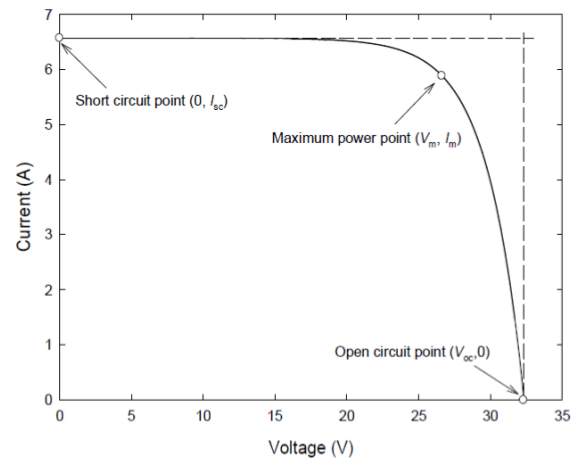
\includegraphics[width=0.4\textwidth]{ivcurve}
%\centering
%\caption{$ I-V $ characteristic curve of an ideal PV cell (Source: \cite{Saloux})}
%\label{fig:ivcurve}
%\end{figure}
%
%Hence, the short-circuit current, the open-circuit voltage, the maximum power voltage and current are written as defined by \cite{Saloux} and shown from Equations \ref{eq:Isc} to \ref{eq:Im}.
%\begin{equation}
%\label{eq:Isc}
%I_{sc}=I_{ph}\vert_{V=0}
%\end{equation}
%
%\begin{equation}
%\label{eq:Voc}
%V_{oc}=\dfrac{aNk_{B}T}{q}ln\left( 1+\dfrac{I_{sc}}{I_{0}} \right) 
%\end{equation}
%
%\begin{equation}
%\label{eq:exp}
%exp\left( \dfrac{qV_{oc}}{aNk_{B}T} \right) = \left(1+\dfrac{qV_{m}}{aNk_{B}T} \right) exp \left( \dfrac{qV_{m}}{aNk_{B}T} \right) 
%\end{equation}
%
%\begin{equation}
%\label{eq:Im}
%I_{m} =I_{ph}-I_{0}\left[ exp \left( \dfrac{qV_{m}}{aNk_{B}T} \right) -1 \right] 
%\end{equation}
%
%Equation \ref{eq:exp} is not explicit with the PV key parameters, therefore need to be rewritten in a different way. 
%
%A PV cell has a hybrid behavior, i.e., a current-source at the short-circuit point and voltage-source at the open-circuit point \cite{Saloux}. 
%These two regions are characterized by two asymptotes of the $ I-V $ curve in Fig. \ref{fig:ivcurve}, where the transition is a compromise between both behaviors. It is interesting to observe that the maximum power point corresponds to a trade-off condition, where the current is still high enough before it starts decreasing with increasing the output voltage (Fig. \ref{fig:ivcurve}).
%
%Based on this, the tangent of the I-V curve can be used to evaluate the transition between current- to voltage-source controlled regions; this operation yields Equation \ref{eq:didv}.
%
%\begin{equation}
%\label{eq:didv}
%\dfrac{dI}{dV}=-\dfrac{qI_{0}}{aNk_{B}T}exp \left( \dfrac{qV}{aNk_{B}T}  \right) 
%\end{equation}
%
%The derivative of Equation \ref{eq:didv} is used to calculate the output voltage that corresponds to the maximum power operation condition of the cell. Therefore, the Equation \ref{eq:Vmderiv} is generated.
%
%\begin{equation}
%\label{eq:Vmderiv}
%V_{m}=\dfrac{aNk_{B}T}{q} ln \left( -\dfrac{qNk_{B}T}{qI_{0}} \left( \dfrac{dI}{dV}  \right)_{V_{m}}   \right) 
%\end{equation}
%
%It is evident that Equation \ref{eq:Vmderiv} requires an expression of the derivative of the current with voltage evaluated at the maximum power point. The fact that the maximum power corresponds to an extreme, the variation of the maximum output power with voltage is relatively small, i.e., a change on $ V_{m} $ has a relatively small effect on the maximum power of the cell \cite{Saloux}. Consequently, considering the asymptotic behavior of the $I-V$ curve at short- and open-circuit conditions, the derivative required by Equation \ref{eq:Vmderiv} can be calculated as shown in Equation \ref{eq:dIdV_Vm}.
%
%\begin{equation}
%\label{eq:dIdV_Vm}
%\dfrac{dI}{dV}\vert_{V_{m}} \cong -\dfrac{0-I_{sc}}{V_{oc}-0}=\dfrac{I_{sc}}{V_{oc}}
%\end{equation}
%
%Replacing the Equation \ref{eq:dIdV_Vm} into Equations \ref{eq:Vmderiv} and \ref{eq:Im}, 
%
The voltage and the current at the maximum power point tracking (MPPT), can be described by Eq. \eqref{eq:Vmfinal}, and Eq. \eqref{eq:Imfinal}~\cite{Saloux}: %, and Eq. \eqref{eq:Pm} as follows~\cite{Saloux}: %These equations are used to calculate the key cell parameters at the maximum power point as function cell temperature and parameters from the manufacturer's data-sheet.
\begin{equation}
\label{eq:Vmfinal}
V_{m}=\dfrac{aNk_{B}T}{q} ln \left( \dfrac{aNk_{B}T}{qI_{0}} \dfrac{I_{sc}}{V_{oc}}  \right). 
\end{equation}

\begin{equation}
\label{eq:Imfinal}
I_{m} = I_{ph} + I_{0} - \dfrac{aNk_{B}T}{q} \left( \dfrac{I_{sc}}{V_{oc}} \right).  
\end{equation}

%\begin{equation}
%\label{eq:Pm}
%P_{m} = V_{m} I_{m}.
%\end{equation}
%
%\begin{multline}
%\label{eq:Pm}
%P_{m} = V_{m} I_{m} = \left[ \dfrac{aNk_{B}T}{q} ln \left( \dfrac{aNk_{B}T}{qI_{0}} \dfrac{I_{sc}}{V_{oc}}  \right) \right] \times \\ \left[ I_{ph} + I_{0} - \dfrac{aNk_{B}T}{q} \left( \dfrac{I_{sc}}{V_{oc}} \right)  \right] 
%\end{multline}
%
However, the photo-current delivered by the constant current source ($I_{ph}$) or even the reverse saturation current ($ I_{0} $) are not given by PV manufacturers. Therefore, Eq. ~\eqref{eq:Iph} is used to calculate the photo-current as function of irradiance and temperature~\cite{Villalva}:
\begin{equation}
\label{eq:Iph}
I_{ph}=\dfrac{G}{G_{ref}} \left[ I_{ph,ref} + \mu_{I} \left( T-T_{ref} \right)    \right], 
\end{equation}

\noindent where the reference state (STC) of the cell is given by the solar irradiance $ G_{ref}=1000\:W/m^{2} $ and the temperature $ T_{ref}=298.15 K (=25^{o}\:C) $; $ \mu_{I} $ is the short-circuit current temperature coefficient ($A/K$); %and corresponds to the photocurrent obtained from a given PV cell working at reference conditions.
$ I_{ph,ref} $ can be approximated to the reference short-circuit current ($ I_{sc,ref} $)\cite{Villalva}.
% that is provided by PV manufacturers ($ I_{sc,ref} $).
%\cite{Jakhrani} that is provided by PV manufacturers ($ I_{sc,ref} $).
%%
The cell temperature ($ T $) in degree Celsius is described by Eq. \ref{eq:Tcell}~\cite{Ross}:
\begin{equation}
\label{eq:Tcell}
T = T_{air} + \dfrac{NOCT-20}{800}G,
\end{equation}

\noindent where $ T_{air} $ is the ambient temperature, $NOCT$ is the nominal operating cell temperature (in $^{o}$C), and $G$ is the solar irradiance ($ W/m^{2} $) of the place where the PV system is deployed.

Furthermore, Eq. ~\eqref{eq:I0} permits the saturation current ($ I_{0} $) to be expressed as a function of the cell temperature as~\cite{Villalva} 
%In this study, this relation is explicitly written based on cell open-circuit conditions using the short-circuit current temperature coefficient as well as the open-circuit voltage temperature coefficient (Equation \ref{eq:I0}).

\begin{equation}
\label{eq:I0}
I_{0} = \dfrac{I_{sc,ref} + \mu_{I}(T - T_{ref})}{exp \left[ \dfrac{q(V_{oc,ref} + \mu_{V} (T - T_{ref}))}{aNk_{B}T}    \right] -1},
\end{equation}

\noindent where $ V_{oc,ref} $ is the reference open-circuit voltage and $ \mu_{V} $ is an open-circuit voltage temperature coefficient ($ V/K $).

%The ideality (or quality) factor of the diode $ a $, which is usually considered as a constant \cite{Villalva}, is determined in the reference state. 
Using the maximum power point current, cf. Eq.~\eqref{eq:Imfinal}, and the saturation current in the reference temperature given by Eq.~\eqref{eq:I0}, the diode ideality factor~\cite{Saloux} is determined by Eq.~\eqref{eq:a}:
\begin{equation}
\label{eq:a}
a = \dfrac{q(V_{m,ref}-V_{oc,ref})}{Nk_{B}T} \dfrac{1}{ln \left( 1 - \dfrac{I_{m,ref}}{I_{sc,ref}}  \right) },
\end{equation}

\noindent where $V_{mref}$, $V_{oc,ref}$, $I_{m,ref}$, and $I_{sc,ref}$ are key cell values obtained under both actual cell temperature and solar irradiance conditions. %, usually provided by manufacturers; t

%The PV generator model is now completely determined; it requires the actual cell temperature (or the air temperature), the actual solar irradiance and common data provided by manufacturers in data-sheets or manuals.
%
%If the PV cells are in parallel, then there is a parallel array. Therefore, there will be a change at the $ I_{ph} $ and $ I_{0} $and the resulting current is given by Equation \ref{eq:Iarray}, as demonstrated in \cite{Saloux}.
%
%\begin{equation}
%\label{eq:Iarray}
%I_{array} = (N_{cells in parallel})(I_{one cell})
%\end{equation}
%
%Where $ I_{one cell} $ is the current from Equation \ref{eq:Imfinal}.
%
%In addition, if the panels are in series, the current do not change but the total voltage is the sum of the each panel's voltage.
%
%\begin{equation}
%\label{eq:Varray}
%V_{array} = (N_{cells in series})(V_{one panel})
%\end{equation}
%
%Where $ V_{one panel} $ is the voltage from Equation \ref{eq:Vmfinal}.
%------------------------------------------------------------
%Because of the fluctuating nature of the output delivered by the PV arrays, batteries are nece\sqrt{•}ry in a PV system. Thus, during the hours of sunshine, the PV system feeds directly the load and the excess electrical energy is stored in the battery. During the night, or during a period with low solar irradiation, energy is supplied to the load from the battery \cite{Mellit}.
  
Related to the \textbf{batteries}, various models have been described in the literature and the most common ones are based on lead-acid batteries~\cite{Copetti,Pinho};
%, and \cite{Manwell93, Manwell94}. 
%However, regardless of the model, normally the following parameters are required: 
%
%\begin{itemize}
%\item Nominal capacity ($ q_{max} $), is the number of Ampere-hours ($ Ah $) that can maximally be extracted from the battery
%, under predetermined discharge conditions.
%\item State of charge ($ SOC $), is the ratio between the present capacity and the nominal capacity, i.e., $ SOC = q/q_{max} $. 
%Obviously $ 0<SOC<1 $. 
%If $ SOC=1 $, then the battery is totally charged; and if $ SOC=0 $, the battery is fully discharged
%\item Charge (or discharge) regime.This parameter reflects the relationship between the nominal capacity of a battery and the current at which it is charged (or discharged). 
%It is expressed in hours: for instance, discharge regime is 30h for a battery of 150 Ah that is discharged at 5A.
%\item Efficiency ($\eta_{b}$), is the ratio of the charge extracted during discharge divided by the amount of the charge needed to restore the initial state of charging or discharging current. 
%\item Lifetime, is the number of charge/discharge cycles the battery can sustain before losing 20\% of its nominal capacity.
%\end{itemize}
%
%The merit of a stand-alone PV system is evaluated in terms of the reliability of the electricity supply to the load and in terms of the long-term efficiency of the components. The battery efficiency was described in this section, and the liability is quantified by the concept of loss of load probability (LLP). LLP is defined as the ratio between the Ampere-hour deficit and the Ampere-hour demand, both with respect to the load, over a long period of time \cite{Copetti}. 
%
%In general, the battery models view the battery as a voltage source $ E $ in series with an internal resistance $ R_{0} $, as shown in Fig. \ref{fig:batteryckt}. 
%
%\begin{figure}[h]
%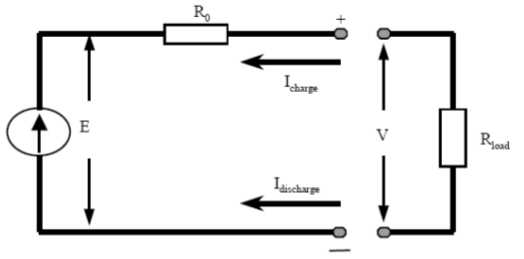
\includegraphics[width=0.4\textwidth]{batteryckt}
%\centering
%\caption{Schematic diagram of the battery (Source: \cite{Hansen})}
%\label{fig:batteryckt}
%\end{figure}
%
%The terminal voltage of the battery can be expressed in terms of its open circuit voltage and the voltage across the internal resistance of the battery \cite{Sukamongkol}, as shown by Equation 31.  
%
%Where $ V_{b} $ is the battery terminal voltage, $ E_{oc} $ is the battery circuit voltage, $ I_{b} $ is the battery current, and $ R_{b} $ is the internal resistance of the battery.
%
%The battery model, which describes the relationship between the voltage, current and the state of charge, can be found in \cite{Copetti}, \cite{Manwell93}, and \cite{Manwell94}.  
%
%The Kinetic Battery Model (KiBaM) of Manwell and McGowen \cite{Manwell93} was developed at the University of Massachusetts to predict the performance of the battery, based on manufacturer's data. However, it uses some data extracted from tested batteries in laboratory. Therefore is not suitable to this study. 
%
that kind of battery has relative low cost and wide availability~\cite{Copetti}. 
%
Here, the model adopted uses only manufacturer's data without empirical tests~\cite{Copetti}. % and allows finding relations among voltage, current, state of charge and temperature. 
%
The discharge voltage is described by Eq. \eqref{eq:bat_Vd}.
%The first term represents the voltage variation with the state of charge ($ SOC $), i.e., the electrolyte concentration, and the second is the variation due to internal resistance variation.
%
\begin{multline}
\label{eq:bat_Vd}
V_{d} = \left[ 2.085-0.12(1-SOC) \right] - \dfrac{I}{C_{10}} \left( \dfrac{4}{1+I^{1.3}} + \dfrac{0.27}{SOC^{1.5}}+0.02 \right) (1-0.007 \Delta T),
\end{multline}

\noindent where $C_{10}$ means 10 h of rated capacity (manufacturer's data-sheet), $\Delta T$ is temperature variation ($\Delta T=T-T_{ref} $%, $ T_{ref}=25^{o}C $
), $ SOC $ or state of charge indicates how much electric charge is stored in the cell at a given time. %Mathematically, it is the ratio between the present capacity and the nominal capacity% (in $ Ah $, provided by manufacturer)
%If $SOC=1$, then the battery is totally charged; and if $ SOC=0 $, then the battery is fully discharged.  %, defined by Equation \ref{eq:SOCbat}.
%\begin{equation}
%\label{eq:SOCbat}
%SOC = \left( 1 - \dfrac{Q}{C} \right) 
%\end{equation}
%
%Where $ Q $ is the charge delivered at the time of interest ($ Q=It $), and C is the battery capacity.
%
%The ratio between $ Q $ and $ C $ represents t
The depth of discharge ($DOD$) or the fraction of discharge, is $DOC=1-SOC$.

%The efficiency of the battery discharge is assumed to be 100\%, according \cite{Copetti}; however, the total amount of useful charge available during discharge is limited by the current rate and temperature given by Equation \ref{eq:CC10}. This equation, called of capacity, is normalized with respect to discharge current corresponding to $ C_{10} $ rated capacity ($ I_{10} $).
%
%\begin{equation}
%\label{eq:CC10}
%\dfrac{C}{C_{10}} = \dfrac{1.67}{1+0.67 \left( \dfrac{I}{I_{10}} \right)^{0.9} }(1+0.005 %\Delta T)
%\end{equation}
%
%Note that when the discharge current tends to zero at 25$^{o}$C, the maximum capacity that can be removed is about 67\% over the capacity.
For the charging process, the parameters are described by Eq.~\eqref{eq:Vcbat} as
%
\begin{multline}
\label{eq:Vcbat}
V_{c} = [2+0.16SOC]+ \dfrac{I}{C_{10}} \left( \dfrac{6}{1+I^{0.86}} + \dfrac{0.48}{(1-SOC)^{1.2}} + 0.036  \right) (1-0.025 \Delta T).
\end{multline}
%
%Note that SOC can be calculated easily at any point during the discharge period, thereby considering the current drained from batteries during a certain time period. %; however, during recharge it is much more difficult \cite{Copetti}.
%Generally, the efficient region is where $ SOC $ is below $ 0.7 $ and $ V_{c} $ is less than $2.3 V$ per cell. The efficiency drops to zero at full charge and the function that represents the charge efficiency ($ \eta_{c} $) variation with state of charge and current rate is given in Equation \ref{eq:efficcharge}.
%\begin{equation}
%\label{eq:efficcharge}
%\eta_{c} = 1 - exp \left[ \dfrac{20.73}{\dfrac{I}{I_{10}}+0.55} (SOC-1) \right] 
%\end{equation}
%
%\cite{Copetti} show that, 
%During overcharge, gassing occur and tests demonstrated that the final charge voltage ($ V_{ec} $) increases with the current intensity and with the decreasing of the temperature (\ref{eq:Vec}). It was created a function for the gassing voltage as well, as shown in (\ref{eq:Vg}). In addition, the overcharge phenomenon can be represented by (\ref{eq:Voverc}).
%\begin{equation}
%\label{eq:Vec}
%V_{ec} = \left[ 2.45 + 2.011 ln \left( 1+\dfrac{I}{C_{10}} \right)  \right] (1-0.002 \Delta T)
%\end{equation}
%
%\begin{equation}
%\label{eq:Vg}
%V_{g} = \left[ 2.24 + 1.97 ln \left( 1+\dfrac{I}{C_{10}} \right)  \right] (1-0.002 \Delta T)
%\end{equation}
%
%\begin{multline}
%\label{eq:Voverc}
%V_{c} = V_{g} + (V_{ec} - V_{g}) \\ \left[ 1- exp \left( \dfrac{Ah_{restored}-0.95C}{I\tau}  \right)    \right] 
%\end{multline}
%
%Where $ Ah_{restored} $ represents the Ampere-hour stored in the battery with regard to the battery capacity ($ C $) during this hour.
%
%The function assumes that 95\% of the capacity was already restored at the start of overcharge.
%
%The time constant of the phenomenon ($ \tau $) is reversely proportional to the charge intensity and can be written by (\ref{eq:tau}).
%\begin{equation}
%\label{eq:tau}
%\tau = \dfrac{17.3}{1+852 \left( \dfrac{I}{C_{10}} \right) ^{1.67} }
%\end{equation}
%
%Therefore, to model the voltage ($ V_{c} $) evolution of the battery, (\ref{eq:Vcbat}) can be used up the start of gassing ($ V_{c} \leq V_{g} $). And during overcharging ($ V_{c} > V_{g} $), (\ref{eq:Voverc}) can be used until a constant final voltage ($ V_{ec} $) is reached.
%
%The storage capacity of the battery can be calculated using Equation \ref{eq:stor}, as defined in \cite{Wenham}.
%
%\begin{equation}
%\label{eq:stor}
%Storage capacity = \dfrac{N_{C}E_{load}}{DOD \eta _{b}}
%\end{equation}
%
%Where $ DOD $ is the maximum possible depth of battery discharge, $ E_{load} $ is the average energy consumed by the load, $ N_{C} $ is the largest number of continuous cloudy days of the area, and $ \eta_{b} $ is the efficiency of the battery.
%
%As an example of this formula application, as shown by \cite{Abdulateef}, considering that a stand-alone PV system is intended to supply $1.5 kW/48 V$ for 24 hours ($=36 kWh$); The largest number of continuous cloudy days in the selected site is about 1 day; For a maximum depth of discharge for the battery $DOD$ of $0.8$ and battery efficiency $80\%$.
%
%Then the storage capacity using Equation \ref{eq:stor} becomes $56.3 kWh$. Since the selected DC bus voltage is $48 V$, then the required Ampere-hours of the battery is $1173 Ah$ ($56.3 kWh/48$). If a single battery of 12 V and 350 Ah is considered, then four batteries are connected in series ($4 \times 350 Ah = 1400 Ah$).
%
%At this research, it was considered a simplified model for charging (Equation \ref{eq:charge}) and discharging (Equation \ref{eq:discharge}) of the batteries, even considering that the process is not linear and depends on the temperature. The equations are used to update the $SOC$ of the batteries, and have the number of hours ($ Num_{h} $) as a variable. There is a factor (1.15) which is present at the charging equation, and is necessary to express that during the charging process is usual to reach 115\% of the battery capacity
%
%\begin{multline}
%\label{eq:charge}
%SOC_{charge} = SOC_{previous} + \\ \dfrac{100*Pm*Num_{h}}{V_{system}*capacity*N_{BP}*1.15}
%\end{multline}
%
%\begin{multline}
%\label{eq:discharge}
%SOC_{discharge} = SOC_{previous} - \\ \dfrac{100*I_{drained}*Num_{h}}{capacity}
%\end{multline}
%
%
%---------------------------------------------------------
%---------------------------------------------------------
%Depending on the literature, the controller can receive different names: controller \cite{Hansen}, charge controller \cite{Mahanta} and \cite{Chauhan}, regulator \cite{Mellit}, DC-DC converter with MPPT and switch \cite{Dhanowa}, \cite{Yatimi}, \cite{Abdulateef}, \cite{Roy}. However, in this study, in order to simplify, the term used is controller. 

The \textbf{charge controller} or controller is the responsible to manage the energy flow to PV system, batteries and loads by collecting information on the battery voltage and knowing the maximum and minimum values acceptable for the battery voltage. Controllers with MPPT mechanism are the mostly used nowadays,  and it maintains the PV operating at the stage of maximum power. %Controllers aim to protect the battery (or batteries) against the excessive charge and discharge \cite{Pinho}, improving its lifetime. 
%
%The resource MPPT, called of maximum power point tracking, is an electronic control mechanism that maintains the PV operating in a voltage that correspond to the voltage of maximum power.
%
%
%As defined by \cite{Hansen} and \cite{Mellit}, all power systems must include a control strategy, which describes the interactions between its components. The use of battery as a storage form implies thus the presence of a charge controller. 
%
%%%%%%%%%%In general, there are two main operating modes for the controller~\cite{Rawat}: normal operating condition, when the battery voltage fluctuates between maximum and minimum voltages; and overcharge or over-discharge conditions, which occur when the battery voltage reaches some critical values. 
%
%The controller allows the management of energy between the load and the battery \cite{Mellit}. 
%The input signals for regulator model are the battery current ($ I_{br} $), PV generator's voltage ($ V_{PV} $), PV generator's current ($ I_{PV} $), and battery voltage ($ V_{b} $). The outputs are battery ($ I_{rb} $) current and used current ($ I_{u} $). 

The steps in the modeling of the controller process are summarized in Table~\ref{table:controller}. To protect the battery against an excessive charge, the PV arrays are disconnected from the system, when the terminal voltage increases above a certain threshold $V_{max \_ off}$ and when the current required by the load is less than the current delivered by the PV arrays~\cite{Hansen}. PV arrays are connected again when the terminal voltage decreases below a certain value $ V_{max \_ on} $. 
%This can be done by using a switch with a hysteresis cycle, as illustrated in Fig. \ref{fig:controllerover}. 
%
%\begin{figure}[h]
%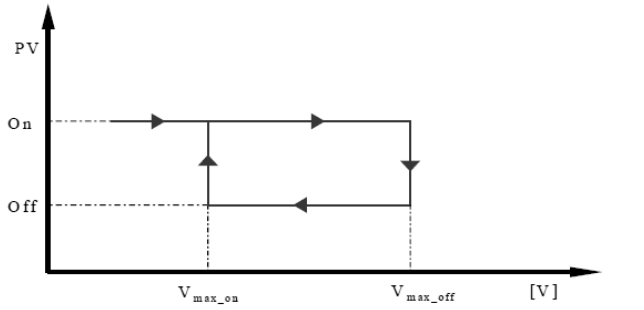
\includegraphics[width=0.4\textwidth]{controllerover}
%\centering
%\caption{Operating principle of an overcharge protector (Source: \cite{Hansen})}
%\label{fig:controllerover}
%\end{figure}
%
In order to protect the battery against excessive discharge, the load is disconnected when the terminal voltage falls below a certain threshold $V_{min \_ off}$ and when the current required by the load is larger than the current delivered by the PV arrays~\cite{Hansen}. The load is reconnected to the system, when the terminal voltage is above a certain value $V_{min \_ on}$.
%, using a switch with a hysteresis cycle, as shown in Fig. \ref{fig:controllerdisc}. 
%
%\begin{figure}[h]
%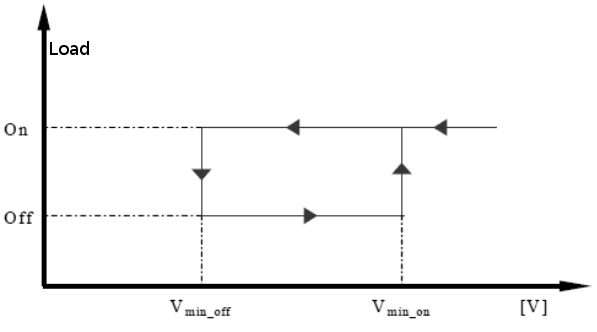
\includegraphics[width=0.4\textwidth]{controllerdisc}
%\centering
%\caption{Operating principle of a discharge protector (Source: \cite{Hansen})}
%\label{fig:controllerdisc}
%\end{figure}
%
%According to \cite{Lorenzo}, the switches may either be electromechanical (relay, contactors, etc.) or solid state (bipolar transistors, MOSFET's, etc.). 
%
\begin{table}[!t]
%% increase table row spacing, adjust to taste
\renewcommand{\arraystretch}{1.3}
% if using array.sty, it might be a good idea to tweak the value of
% \extrarowheight as needed to properly center the text within the cells
\caption{Summary of the controller process (adapted from~\cite{Hansen})}
\label{table:controller}
\centering
%% Some packages, such as MDW tools, offer better commands for making tables
%% than the plain LaTeX2e tabular which is used here.
\begin{tabular}{c | c | c }
\hline
\hline
Step  & Constraint & Command\\
\hline
\hline
(1) & \makecell{If $V > V_{max \_ off}$ \\and $I_{load} < I_{pv}$} & \makecell{Disconnect PV array \\from the system}\\
\hline
(2) & \makecell{If command (1) is \\done and $V < V_{max \_ on}$} & \makecell{Reconnect PV array \\to the system}\\
\hline
(3) & \makecell{If $V < V_{min \_ off}$ and \\ $I_{load} > I_{pv}$} & \makecell{Disconnect the load \\from the system}\\
\hline
(4) & \makecell{If command (3) is \\ done and $V > V_{min \_ on}$} & \makecell{Reconnect the load \\to the system}\\
\hline
\hline
\end{tabular}
\end{table}

%Regarding the DC-DC converter, the most basic idea is that the power is converted while altering the current and voltage. 
%
%As shown in \cite{Abdulateef}, the DC-DC converter is used to increase the efficiency of the PV system by matching the voltage generated by PV array to the voltage required by the load. 
The output power ($ P_{out} $) of controller is given by Eq. \eqref{eq:poutcont}.
\begin{equation}
\label{eq:poutcont}
P_{in} \eta_{c} = P_{out}.
\end{equation}

Assuming that the efficiency of the controller ($ \eta_{c} $) is a manufacturer's data, from Eq. \eqref{eq:poutcont} we compute Eq. \eqref{eq:potcont}.
\begin{equation}
\label{eq:potcont}
V_{in} I_{in} \eta_{c} = V_{out} I_{out},
\end{equation}

\noindent where $ V_{in} $ is the voltage across the PV array, $ I_{in} $ is the output current of PV array, $ V_{out} $ is the  DC bus voltage, and $ I_{out} $ is the output current from the converter.

%The output voltage is related to the input voltage as a function of duty cycle of the switch (\cite{Abdulateef}). 
% 
%A DC-DC converter can either be step-up (Boost), step-down (Buck), or both increase and decrease (Buck-Boost) the voltage, as defined by \cite{Mahanta}. In addition, there is the Cuk converter, which is a Buck-Boost converter with an inverting topology \cite{Catherine}. 
%
%For the Cuk converter, the relationship is expressed by \ref{eq:voutvin} as show in \cite{Abdulateef}.
%
%\begin{equation}
%\label{eq:voutvin}
%\dfrac{V_{out}}{V_{in}} = \dfrac{D}{D-1}
%\end{equation}
%
%Where $D$ is the duty cycle or ratio of the circuit converter, i.e., it is defined as the ratio of the on time of the switch to the total switching period.
% 
%The DC/DC converter should always operate in the MPPT to maximize the PV array efficiency and consequently increase the efficiency of the PV system, as defined in \cite{Yatimi}.
%  
%Various types of MPPT schemes are proposed by researchers, namely open circuit, short circuit, perturb and observe (P\& O)/hill climbing, incremental conductance, and so forth, as shown by \cite{Haque}.
% 
%As the MPPT definition and the equations to get the maximum power from the PV panels was described at the end of the PV panel modeling, the important here is to notice that the Equation \ref{eq:voutvin} defines the relationship between the input signal, the efficiency of the controller and the output power.
 
%The number of controllers required for the stand-alone PV system, as defined by \cite{Yatimi}, is calculated using Equation \ref{eq:numberofcmin}. In addition, the final sizing check is did by Equation \ref{eq:numberofc}, who validate the number of controllers adopted.
%\begin{multline}
%\label{eq:numberofcmin}
%number_{controllers} = \dfrac{Total \, max \, power \, of \, PV}{Controller \, max \, power} = \\ \dfrac{P_{m,ref} \times N_{TP}}{V_{system} \times I_{controller,max}}
%\end{multline}
%
%\begin{equation}
%\label{eq:numberofc}
%N_{controller} \geq number_{controllers}
%\end{equation}
%
%\subsection{Joint work: charge controller and batteries}
%When batteries are charged, they go through three main different states - bulk, absorption and float, with impact to the inverter and to power supplied to the house.
%, and it is necessary to understand those three states in order to comprehend the joint work of the controller with the battery. With impact to the inverter and to power supplied to the house. 
%
%All the explanation at this section is related to $SOC$ and to the voltage at the DC-bus (controller output, which will be bigger than $V_{system}$) where the batteries are connected, all ruled by the charge controller. Moreover, it is important to mention that smart chargers, the most usual nowadays, will detect voltage and resistance from the battery prior to charging.
%
%Bulk - is the first stage of charging. Bulk begins when the sun comes out.
%, or other source of electrical generation is turned on. 
%This stage occurs when the batteries are at a lower $SOC$, generally anything not smaller than $75\%$ to $80\%$ (defined during system sizing). This stage is typically where the highest voltage and current the charger is rated for will actually be used. The bulk stage basically allows the PV panel to put as much current into the batteries as possible. For a typical 12 V battery, the charging voltage going into a battery will reach 14.16 V to 14.40 V at this stage, and there is no risk of overcharging in this stage because the battery hasn't even reached full yet.
%
%Absorption - once the batteries reach the programmed absorb voltage, usually somewhere between 14.16 and 14.40 V, the batteries will go into the absorption stage. Typically, when a battery reaches this stage its $SOC$ is around $85-95\%$. During this stage, the batteries are kept at the programmed voltage, and the current going into the batteries reduces as the batteries become more full. The absorption stage ends after the programmed time is reached or the number of Ampere going into the battery falls below a preset number. The lower current going into the battery safely brings up the charge on the battery without overheating it. 
%Usually, this stage takes more time than the bulk stage.
%
%Float - upon the completion of the absorption stage, the charge controller will  drop down the voltage and maintain at a steady 13.20 V to 13.38 V (manufacturer's defined value), which is the maximum voltage that a 12 V battery can hold, and begin the float stage. The float stage brings the battery all the way through and maintains $SOC$ at $100\%$. The current will also decrease to a point where it's considered just a pulse. It's essentially the float stage where there is charge going into the battery at all times, but only at a safe rate to ensure a full state of charge and nothing more. 
%Most smart chargers do not turn off at this point, however it is completely safe to leave a battery in float mode for months to even years at a time.
%
%Battery charging technology relies on smart micro-controlled devices. Therefore it is extremely important that the program settings for the charge controller or inverter/charger are correct, and the list includes the bulk and absorption values. 
%This will help preserve and extend the battery life. There are always default settings to the equipment, set by software, however those settings are not $100\%$ correct because there are difference among models of equipment and among manufacturer's. The ideal is to read the data-sheet from the manufacturers and perform a manual adjust.
%
%There are the possibility to combine batteries in a bank, with parallel and series connections, all depending the sizing of the project:
%
%\begin{itemize}
%\item Batteries connected in parallel are seen by the controller as one large battery of the combined Ah capacity of all the batteries. For example, two 12 V and 220 Ah batteries in parallel are seen as one 12 V and 440 Ah battery;
%\item In the other hand, although the batteries connected in series are also seen as a single battery, the result is different: two 12 V and 220 Ah batteries in series are seen as one 24 V and 220 Ah battery;
%\item In addition, a mixed bank arrangement can be useful: a bank with two 12 V and 220 Ah batteries in series connected in parallel with a similar arrange will produce an equivalent battery of 24 V and 440 Ah.
%\end{itemize}
%-----------------------------------------------
%-----------------------------------------------
%As shown by \cite{Mellit}, the PV arrays produce DC and therefore when the PV system contains an AC load, a DC/AC conversion is required. 
%An inverter is a converter, where the power flows from DC to AC side, i.e., having a DC voltage as input; it produces AC voltage, as output. 
The role of the \textbf{inverter} is to keep the voltage constant on the AC side, %, i.e., at the rated voltage, % (127 V or 220 V, for example), 
and to convert the input power $ P_{in} $ into the output power $ P_{out} $ with the best possible efficiency $ \eta_{i} $ as described by \eqref{eq:efficinv} \cite{Hansen}:
%
%The inverter is characterized by a power dependent efficiency $ \eta_{i} $ as shown by (\ref{eq:efficinv}) \cite{Hansen}.
\begin{equation}
\label{eq:efficinv}
\eta_{i} = \dfrac{P_{out}}{P_{in}} = \dfrac{V_{AC} I_{AC} cos\varphi}{V_{DC}I_{DC}},
\end{equation}

\noindent where $ I_{DC} $ is the current required by the inverter from the DC source to be able to keep the rated voltage on the AC side, $ V_{DC} $ is the input voltage to the inverter delivered by the DC source (PV panel or battery),  $ V_{AC}  $ and $ I_{AC} $ are the output voltage and current, respectively, and $ cos \varphi $ can be obtained from the inverter's manual.

%Therefore, with this equation it is possible to simulate the output power of the inverter, based on information from the inverter's data-sheet and from the DC module or the PV panel that feed the inverter (which are obtained by this study model). 
%
%
%--------------------------------------------------
\subsection{Availability of Stand-alone PV Systems}
\label{sec:availability}
%--------------------------------------------------
%Each stand-alone PV system, like any other power systems, has a specific level of availability. This reliability level impacts various issues, as system performance, production, feasibility, and investment. 
The availability of a stand-alone PV system can be defined as the percentage of time at which a power system is capable of meeting the load requirements~\cite{Khatib2014}. The number of hours that the system is available, divided by 8,760 h, gives the annual system availability.
The system availability definition depends on how critical the load application is. For critical loads, 99\% is considered acceptable. While in a ordinary house electrical load, 95\% is considered acceptable. %As an example, a system with 95\% availability is expected to meet the load requirement of 8,322 h during an average year for the entire useful life of the system. An annual availability of 99\% means that the system can operate the load for 8,672 h of the 8,760 h.
%
%With that in mind, it is important to mention that even if a formal verification or a simulation shows that a PV system fails, it doesn't mean that the sizing is wrong. It is important to evaluate how critical the load application is and the horizon of evaluation. However this analysis can be useful, for example, to improve the sized battery autonomy.
%
%%%%%%%%%%%%%%%%%%%%%%%%%%%%%%%%%%%%%%%%%%%%%%%%%%%%%%%%


%%%%%%%%%%%%%%%%%%%%%%%%%%%%%%%%%%%%%%%%%%%%%%%%%%%%%%%%
\subsection{Sizing Stand-alone Solar PV Systems}
\label{sec:sizing}
%%%%%%%%%%%%%%%%%%%%%%%%%%%%%%%%%%%%%%%%%%%%%%%%%%%%%%%%

A PV system is illustrated in Fig.\ref{fig:blockdiagram}. It identifies the PV generator, batteries, charge controller, inverter, and AC load. 
The PV generator, which can be a panel or an array, is a semiconductor device that can convert solar energy into DC electricity.  
For night hours or rainy days, we hold batteries where power can be stored and used. The use of batteries as a storage 
form implies the presence of a charge controller~\cite{Hansen}. The PV arrays produce DC and therefore when the PV system 
contains an AC load, a DC/AC conversion is required. That converter is called inverter; and the AC load dictates the behavior 
of AC electrical load from the house that will be fed by the system.
%
\begin{figure}[h]
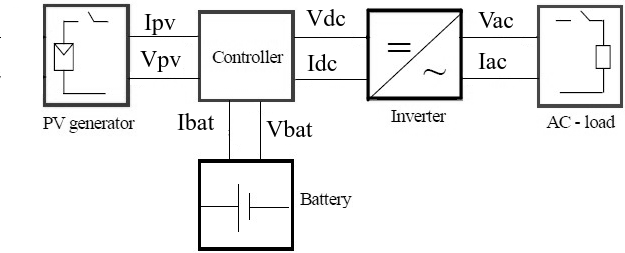
\includegraphics[width=0.7\textwidth]{blockdiagramPVS2_rev}
\centering
\caption{Block diagram for a typical stand-alone PV system~\cite{Hansen}.}
\label{fig:blockdiagram} 
\end{figure}

The sizing check stage will ensure that the system meets the standard project steps related 
to critical period solar energy method~\cite{Pinho} and adopting MPPT (Maximum Power Point Tracking) charge controller,
which is the most common one in practice. Firstly, we need to correct the energy consumption estimated to the load 
($E_{consumption}$), which is carried out by Eq.~\eqref{eq:Ecorrected}, where the efficiency of batteries ($\eta_{b}$), 
controller ($\eta_{c}$), and inverter ($\eta_{i}$) are considered~\cite{Pinho} as follows
%
\begin{equation}
\label{eq:Ecorrected}
E_{corrected} = \dfrac{E_{consumption}}{\eta_{b} \eta_{c} \eta_{i} }.
\end{equation}

We also need to estimate the energy that can be produced for each panel, called $E_{p}$, in Wh, defined as
%
\begin{equation}
\label{eq:Ep}
E_{p} = Solar\_Irradiance \times Panel\_Area \times \eta_{p} \times 1000,
\end{equation}

\noindent where the solar irradiance is expressed in terms of $kWh/m^{2}$ and depends on the site where the PV system will be deployed; 
the PV panel area is given in $m^{2}$ and corresponds to the size of one PV panel, and $\eta_{p}$ represents the PV panel efficiency.
The total minimum number of needed solar panels ($N_{TPmin}$) is computed as
%
\begin{equation}
\label{eq:NTPmin}
N_{TPmin} = \dfrac{E_{corrected}}{E_{p}}.
\end{equation}

Particularly, the total number of panels in series ($N_{PSmin}$) and parallel ($N_{PPmin}$) are respectively given by
%
\begin{equation}
\label{eq:NPSmin}
\dfrac{V_{mppt,min}}{V_{maxPower,TempMax}} \leq N_{PSmin} \leq \dfrac{V_{mppt,max}}{V_{maxPower,TempMin}},
\end{equation}
%
\begin{equation}
\label{eq:NPPmin}
N_{PPmin} = \dfrac{P_{total}}{Number\,Panels\,Series \times P_{max,ref}},
\end{equation}
%
\noindent where $V_{mppt,max}$ is the maximum operation voltage and $V_{mppt,min}$ 
is the minimum operation voltage of the charge controller; $V_{maxPower,TempMax}$ and 
$V_{maxPower,TempMin}$ are the maximum power voltage from the PV module considering 
the maximum and minimum operational temperature, respectively; 
$P_{total}$ is the total power demanded from the PV system and 
$P_{max,ref}$ is the power supplied from one PV panel in $Watts$.
Regarding batteries, we must first define the total capacity of the battery bank, which can be described as
%
\begin{equation}
\label{eq:Cbank}
C_{bank} = \dfrac{E_{corrected} \times autonomy}{V_{system} \times DOD},
\end{equation}

\noindent where the variable $autonomy$ is a design definition and normally has a value ranging from $6$ to $48$h; 
$ V_{system} $ is the DC voltage of the bus, and $ DOD $ is the battery deep of discharge (considered of maximum of 25\% here).
%
Secondly, the total (minimum) number of batteries is computed as 

\begin{equation}
\label{eq:Nbtotal}
N_{B}total = N_{BS}min \times N_{BP}min = \dfrac{V_{system}}{V_{bat}} \times \dfrac{C_{bank}}{1 \,Battery \, Capacity}.
\end{equation}

Regarding the charge controller, it must initially meet the voltage requirement of the PV system, as described by Eq.~\eqref{eq:vcvsystem} to the charge controller voltage: 
\begin{equation}
\label{eq:vcvsystem}
V_{c} = V_{system}.
\end{equation}

The short circuit reference information from the manufacturer's solar panel must be corrected 
to the cell temperature because the field temperature is higher than the nominal or laboratory temperature, 
and PV system is temperature dependent, as 
%
\begin{equation}
\label{eq:iscamb}
I_{sc,amb} = \dfrac{G}{G_{ref}} \left[ I_{sc,ref} + \mu_{I} \times (T-25) \right]. 
\end{equation}

The controller must meet the maximum current from the PV array given by Eqs.~\eqref{eq:icmin} and~\eqref{eq:icicmin} as
%
\begin{equation}
\label{eq:icmin}
I_{c,min} = I_{sc,amb} \times N_{PP},
\end{equation}
%
\begin{equation}
\label{eq:icicmin}
I_{c} \geq I_{c,min}.
\end{equation}

The inverter sizing check is performed by means of three equations. Eq.~\eqref{eq:vindc} ensures that 
the input voltage of the controller meets the system voltage. Eq.~\eqref{eq:voutac} ensures that the 
output voltage of the controller meets the AC voltage of the load. Finally, Eq.~\eqref{eq:invcheck} ensures that 
the controller can support the total demand of the load ($Demand$) and the surge power ($P_{surge}$), 
where $V_{in}DC$ is the nominal input voltage and $V_{out}AC$ is the nominal output voltage of the inverter; 
$MAX_{AC,ref}$ is the peak power that the inverter can support.
%
\begin{equation}
\label{eq:vindc} 
V_{in}DC = V_{system}.
\end{equation}
%
\begin{equation}
\label{eq:voutac} 
V_{out}AC = V_{AC}.
\end{equation}
%
\begin{equation}
\label{eq:invcheck} 
\left[ (Demand \leq P_{AC,ref}) \, and \, (P_{surge} \leq MAX_{AC,ref}) \right].
\end{equation}

%%%%%%%%%%%%%%%%%%%%%%%%%%%%%%%%%
\subsection{PV systems Optimization Criteria}
%%%%%%%%%%%%%%%%%%%%%%%%%%%%%%%%%

In order to select an optimal combination to meet sizing constraints, 
it is necessary to evaluate power reliability and system cost analysis for the underlying system. An ideal combination of any PV system is made by the best compromise between these two objectives.

During the PV system design, one of the most important aspects to ensure power system reliability is to analyze power supply availability~\cite{Alsadi2018}. The reason is because solar energy production is intermittent and, therefore, the energy generated usually will not match with the load demand. A reliable power is a generation system that has sufficient power to feed load demand in a period. 

There exist different methods to express system reliability, where the most popular ones 
are the loss of load probability (LOLP) and the loss of power supply probability (LPSP)~\cite{Alsadi2018}. In both methods, if the probability is zero, then the load will always be fulfilled; otherwise (i.e., probability of one) the load will never be fulfilled.

LOLP is the probability for the case when a load demand exceeds the generation power by the PV system. On one hand, we claim that we have a reliable PV system when it is able to generate sufficient power to fulfill the demanded load within a time span. On the other hand, LPSP is defined as the probability of the case when system generates insufficient power to satisfy the load demand. The main approaches to LPSP demand simulation or probabilistic treatment of time series data to predict dynamic changing on system performance. However, data is not always available and dynamic analysis is complex; and this is a drawback of LOLP and LPSP~\cite{Alsadi2018}.

Related to economic analysis, there exist various methods available. The main objective is to determine whether the project has an acceptable investment; the usual way is to perform economic analysis after reliability analysis with the goal of proposing a system with high reliability and lowest cost~\cite{Alsadi2018}. The common methods include: Net Present Cost (NPC)~\cite{Park2004}, the Levelized Cost of Energy (LCOE)~\cite{Zhou2010}, or the Life Cycle Cost (LCC)~\cite{Applasamy2011}.

The NPC is the present value of all the costs over the project lifetime, minus the present value of all the revenues that it earns over the project lifetime. The net present worth is found by discounting all cash inflows and outflows, including cost of installation, replacement and maintenance of the PV system, at an internal rate of return (IRR)~\cite{Park2004}. IRR is used to evaluate the attractiveness of a project or investment.

LCOE is defined as the average cost per kWh of useful electrical energy produced by the PV system when a lifetime, investment cost, replacement, operation and maintenance, and capital cost are considered~\cite{Kamel2005}. LCOE method is useful in comparing different generation technologies with different operating characteristics~\cite{Zhou2010}.

LCC is the estimation of sum of installation cost, operating and maintenance of a PV system for a period of time, and expressed in today's value~\cite{Applasamy2011}. Eq.~\eqref{eq:LCC} is used to calculate LCC of a PV system,
%
\begin{equation}
\label{eq:LCC}
LCC = C_{PV} + C_{bat} + C_{charger} + C_{inv} + C_{installation} + C_{batrep} + C_{PWO\&M},
\end{equation}
\noindent where $C_{PV}$ is PV array cost, $C_{bat}$ is initial cost of batteries, $C_{charger}$ is cost of charger, $C_{inv}$ is inverter cost, $C_{installation}$ is installation cost, $C_{batrep}$ is battery replacement cost in present value, and $C_{PWO\&M}$ is operation and maintenance costs 
in present worth.

%----------------------------------------------------------------------------------------------
\subsection{Stand-alone PV System Optimization Technique}
%----------------------------------------------------------------------------------------------

In order to recommend an optimal configuration for PV systems, 
the designer has to evaluate the design based on optimization variables. 
As the number of optimization variables increases, the computational effort 
will increase as well. Hence, to obtain the best PV system design as well as 
simplified sizing process, prior work introduced three main techniques 
for system sizing calculation, namely intuitive, numerical, and analytical methods~\cite{Zhou2010}.

Intuitive method is simple, easy to be implemented, and can be used to give 
rough suggestion for preliminary design. The sizing rules are based on designer's experience, 
using lowest performance either in a time period data or by directly using average value 
(daily, monthly, or annual) of solar irradiance. This method does not consider the battery's 
state of charge, or even the random nature of solar irradiation and meteorological conditions~\cite{Alsadi2018}.

For numerical method, the design is simulated for each time step within a period. 
State of charge of batteries is calculated and investigated. It is very accurate, 
however is complex, demanding more time for calculation~\cite{Park2004}.

Analytical methods is used to obtain a close relation or correlation in a form 
of equation between capacities and reliabilities. The sizing task becomes much simpler 
than numerical technique; however, the relation cannot be applied to different sites
since it is specific to one place of deployment of the PV system, 
thereby demanding adaptation if another site is analyzed.

\section{Summary}
